\documentclass[11pt, english]{article}
\usepackage[a4paper, total={15cm, 20cm}]{geometry}
\usepackage[style=authoryear, autocite=inline, maxcitenames=3, maxbibnames=3, uniquename=false, backend=biber]{biblatex}
\usepackage[utf8]{inputenc}
\usepackage{fancyhdr}
\usepackage{graphicx}
\usepackage[onehalfspacing]{setspace}
\usepackage{hyperref}
\usepackage{array} % For table formatting
\hypersetup{
    colorlinks,
    citecolor=black,
    filecolor=black,
    linkcolor=black,
    urlcolor=black
}

\setlength{\parindent}{0pt} % Kein Einzug am Anfang eines Absatzes
\setlength{\parskip}{0.75em} % Abstand zwischen Absätzen

% Customize Inline Citation Format
\renewcommand*{\finalnamedelim}{/} % Change "and" to "/"
\renewcommand*{\multinamedelim}{/} % Change ", " to "/"

% Define Custom Citation Commands
\newcommand{\vglcite}[2][]{(vgl. \cite[#1]{#2})}
\newcommand{\directcite}[2][]{(\cite[#1]{#2})}

% Customize Name Formatting in Bibliography
\DeclareNameAlias{author}{family-given} % Ensure "Last, First" format

% Remove ISBN, pages and series
\AtEveryBibitem{
  \clearfield{isbn}
  \clearfield{pagetotal}
  \clearfield{series}
}

% Customize Bibliography Author Format
\renewbibmacro*{author}{%
  \printnames{author}: 
}

\renewbibmacro*{publisher+location+date}{%
  \printlist{location}:
  \iflistundef{publisher}
    {}
    {\setunit*{\addspace}\printlist{publisher}}%
  \setunit*{\addspace}%
  \printfield{year}
}

% Load Bibliography
\addbibresource{citations.bib}
\graphicspath{{images}}

% Customize Page Style
\pagestyle{fancy}
\fancyhf{}
\fancyhead[LE, LO]{\leftmark}
\fancyfoot[RE, RO]{Page \thepage}
\onehalfspacing


\begin{document}

% \begin{figure}[h!]
% \begin{center}
%     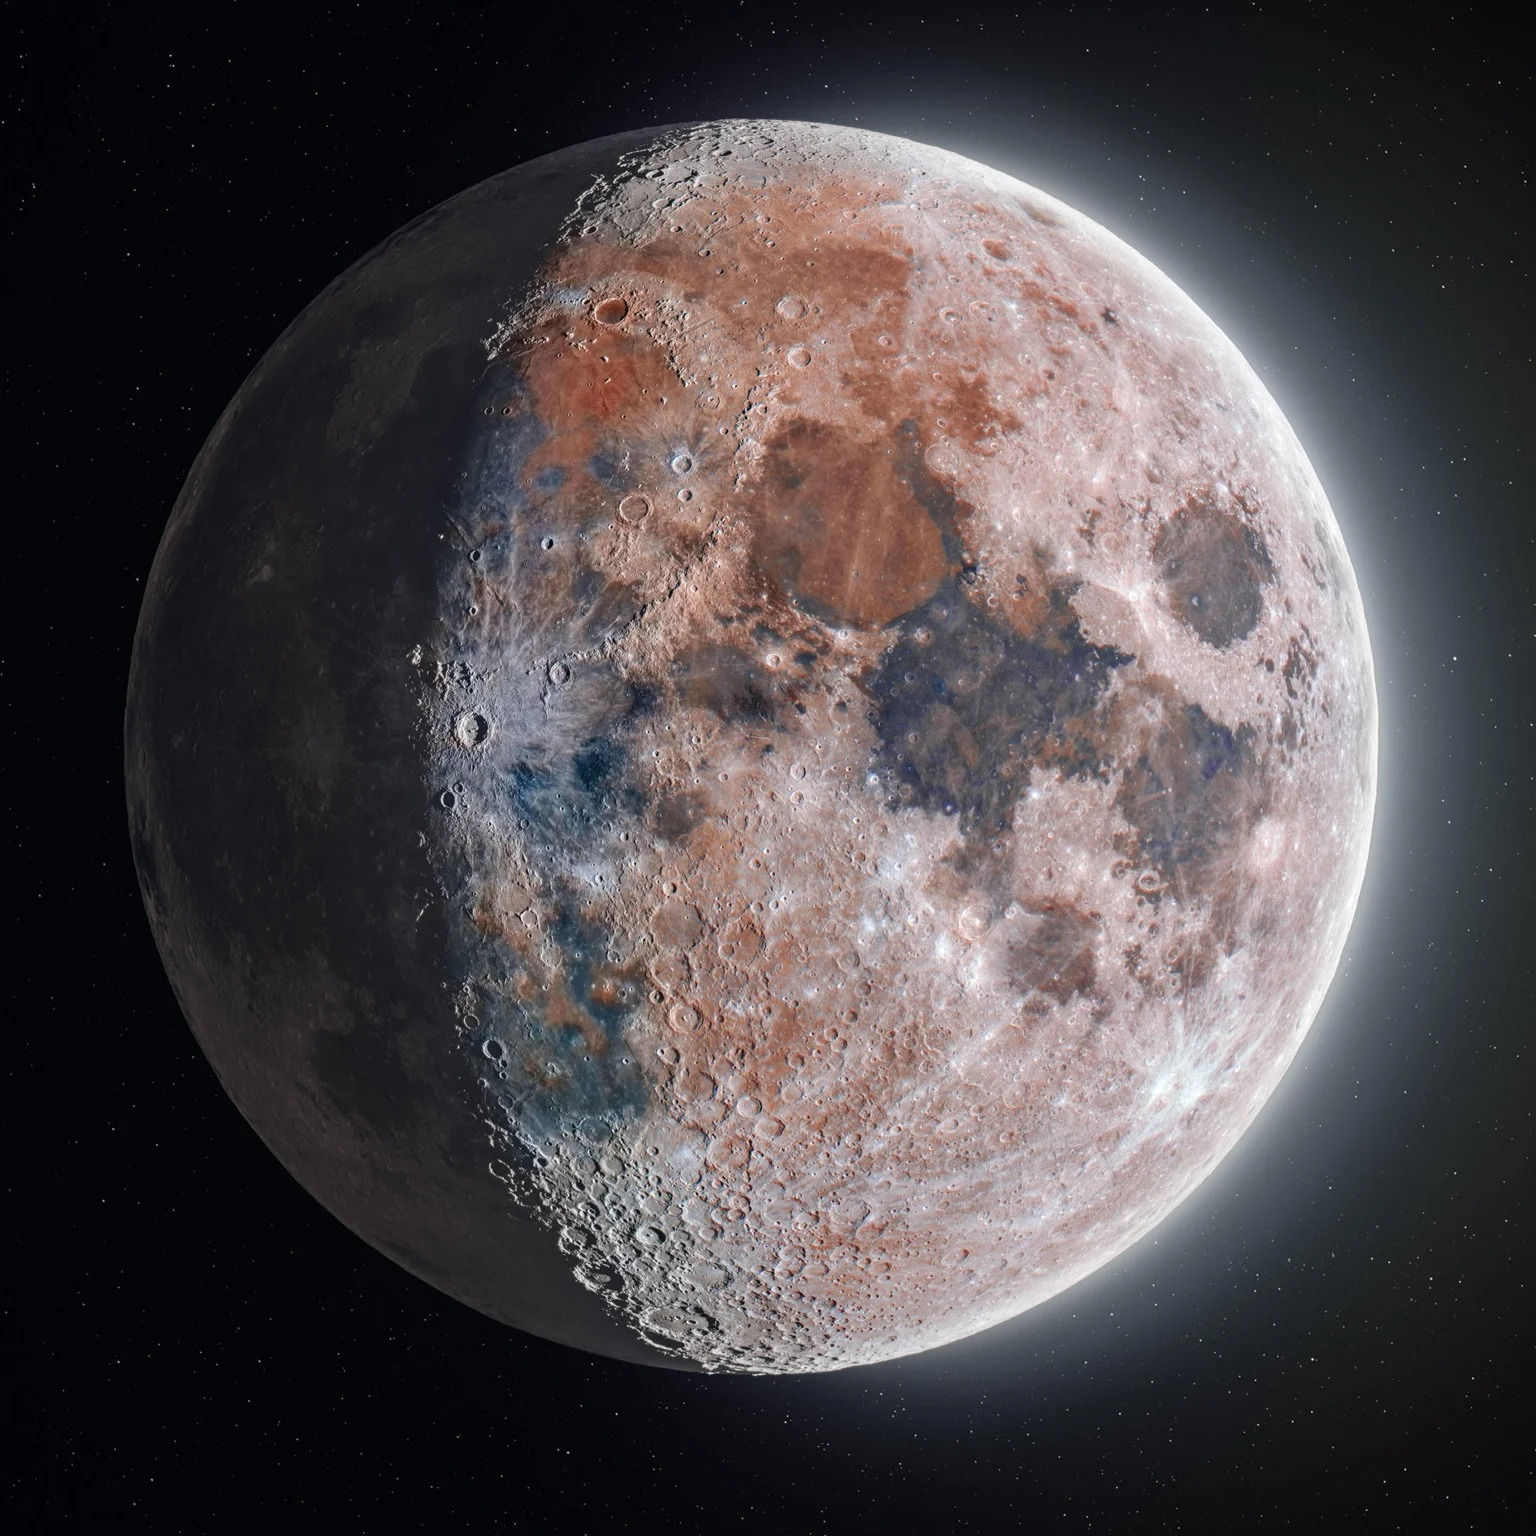
\includegraphics[width=300pt, height=\textheight,keepaspectratio]{test.jpg}
%     \caption[Caption (url)]{Caption visible}
% \end{center}
% \end{figure}

% =============== ABSTRACT ===============

\newpage
\section*{Abstract}
In recent years, web-development has become a fast-paced landscape. For high-quality digital
products, close collaboration between user interface design and development is essential. In
practice, however, misunderstandings and inefficiencies arise, leading to a worse user experience
and demoralized teams.

This bachelor's thesis explores how design workflows and practices can be adapted to better align
with the needs of developers working in small, iterative teams. Based on a strong theoretical
foundation and qualitative insights from surveys and interviews, the thesis presents a practical
educational solution. Its goal is to improve design-to-code workflows by building shared
understanding, establishing common principles and enhancing communication.

\section*{Kurzfassung}
In den letzten Jahren hat sich die Web-Entwicklung zu einem schnelllebigen Feld entwickelt. Für
hochwertige digitale Produkte müssen User Interface Design und Entwicklung eng zusammenarbeiten. In
der Praxis führen jedoch Missverständnisse und ineffiziente Prozesse häufig zu einer
schlechteren User Experience und demotivierten Teams.

Diese Bachelorarbeit untersucht, wie Design-Prozesse und Methoden so angepasst werden können, dass
sie den Anforderungen von Entwickler:innen in kleinen, iterativen Teams besser gerecht werden.
Basierend auf einer soliden theoretischen Grundlage sowie qualitativen Erkenntnissen aus Umfragen
und Interviews wird eine lehrreiche und praxisorientierte Lösung vorgestellt. Ziel ist es,
Design-to-Code-Prozesse durch ein gemeinsames Verständnis, klare Prinzipien und die Förderung von
Kommunikation nachhaltig zu verbessern.


% =============== ABSTRACT ===============


% =============== TABLE OF CONTENTS ===============

\tableofcontents

% =============== TABLE OF CONTENTS ===============


% =============== CHAPTERS ===============

\section{Introduction}


\newpage
\section{Basics of Webdesign}
Optimizing the workflow from User Interface Design to code implementation requires to have a solid
foundational understanding of what UI Design and development is. More specifically, understanding
web-specific aspects of these fields is crucial to optimize the workflow for web projects. In this
chapter, we will discuss the basics of User Interface Design.

\newpage
\subsection{User Interface Design}
The interaction design foundation defines User Interface (UI) Design as "the process designers use
to build interfaces in software or computerized devices, focusing on looks or style. Designers aim
to create interfaces which users find easy to use and pleasurable. UI design refers to graphical
user interfaces and other forms—e.g., voice-controlled interfaces."
\directcite{interactiondesignfoundation-ixdfWhatUserInterface2016}.

This definition is a good starting point to understand what UI design is about, since it
shows that it is about more than just the visual. User interfaces are everywhere, be it an ATM, a
stove, a bike computer or a time tracking app in the browser. Each one of them needs to be
carefully designed. It is about finding ways to make this human-computer interaction as smooth,
efficient and delightful as possible.
\vglcite{interactiondesignfoundation-ixdfWhatUserInterface2016}

\subsubsection{Web Design}
Web Design is a subset of UI Design that specifically focuses on designing websites. While other UI
Design fields often focus on specific platforms, web designers have to consider a wide range of end
user devices like desktop PCs, tablets or smartphones. The practice of adapting and optimizing for
these various screen sizes and aspect ratios is known as \textit{Responsive Design}. Additionally,
\textit{Web Accessibility} is a fundamental aspect of Web Design. It ensures that people with
disabilities can navigate and interact with websites as effectively as possible.
\vglcite{interactiondesignfoundation-ixdfWhatWebDesign2016}

With the European Accessibility Act (EAA) coming into effect in June 2025, this becomes even more
important, as businesses need to comply with stricter regulations on all of their websites.
\vglcite{kleeAccessibilityAct20252024}

Although Web Design is often thought of as a purely visual discipline, when in reality it is a much
more multidisciplinary field. They have to work closely with developers and often know a great deal
of content strategy, information architecture, user research and more. Product designer Mark Boulton
emphazises that "You can create good experiences without knowing the content. What you can’t do is
create good experiences without knowing your content structure. What is your content made from, not
what your content is." \directcite[]{boultonStructureFirstContent2012}

\subsubsection{User Experience and Usability}
Zooming out of the context of User Interfaces is essential to fully understand the concept of User
Experience (UX). UX is about looking at all kinds of touchpoints a user has with a product or
service and seeing the holistic experience. This of course includes the UI, but encompasses several
other domains such as content quality, customer support, branding, and more.
\vglcite{normanDefinitionUserExperience1998}

In other words, even an app like Spotify with a great interface, would have a poor UX if there were
only 10 songs available.

Usability on the other hand is, as Jacob Nielsen suggests, a quality attribute of Interfaces. This
attribute indicates how easy it is for users to use a product, by observing and measuring the five
quality components: learnability, efficiency, memorability, errors, and satisfaction
defined by Nielsen. Additionally, Nielsen introduces another concept that when combined with
usability is an indicator for the overall usefulness of a product - utility. Utility refers to
whether a product offers the necessary features that a user actually needs. Both usability and
utility are crucial for a successful product. Simply having an intuitive interface is of no use if
the product lacks the necessary features, similarly, a product with a fitting feature-set is
ineffective if users struggle navigating it.
\vglcite{nielsenUsability101Introduction2012}
% NOTE DONE: Potential for graphic here (Vann Diagram)
\begin{figure}[H]
    \centering
    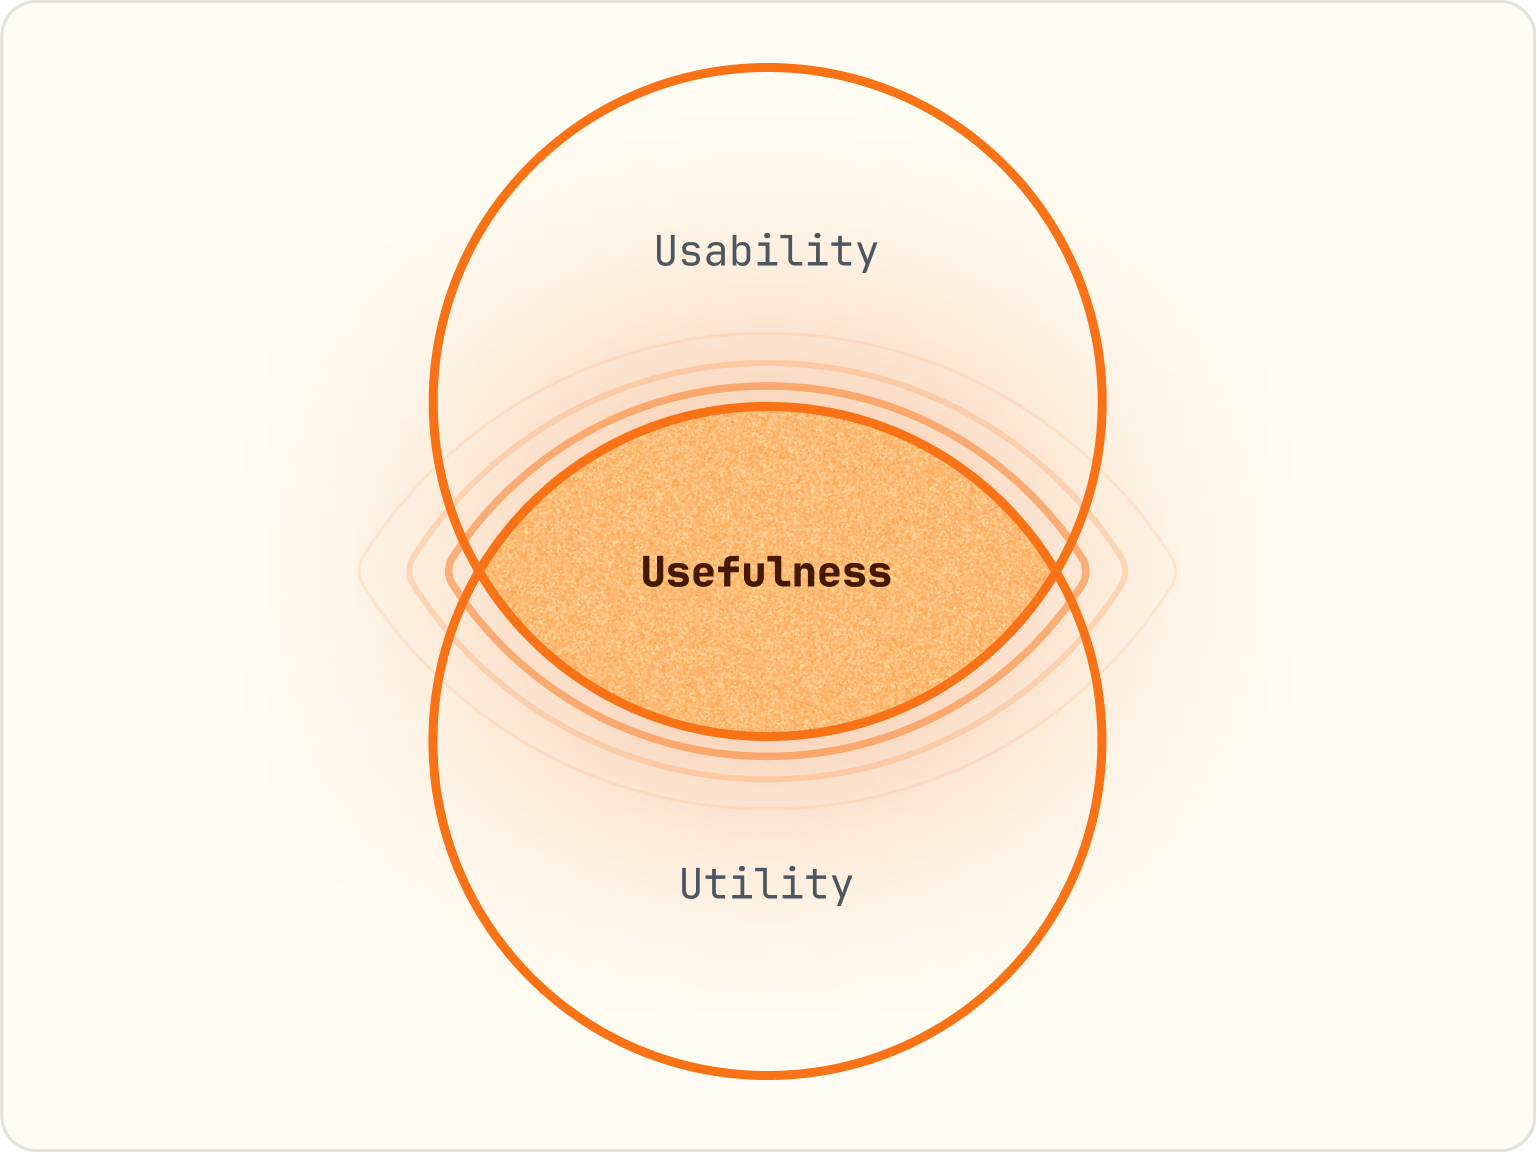
\includegraphics[height=250pt]{Chapter 2/Usefulness.png}
    \caption{Combination of usability and utility according to Jacob Nielsen (Source: own illustration)}
\end{figure}

\subsubsection{Tools}
There are many great tools available that aim to make User Interface Design easier and more
efficient. Some of them also have features that help to bridge the gap between design and code. The
selection of tools is based on their popularity, since the aim is to provide a solution that
tailors to the majority of designers and developers. % NOTE DONE: Add graphic showing the popularity of
% tools (https://uxtools.co/survey/2023/ui-design/#ui-design-yoy-graph)

% NOTE DONE: Add Logo graphic for each of the tools
\textbf{Figma}\\
\begin{figure}[H]
    
\includegraphics[height=50pt]{Chapter 2/Figma.png}
    \caption{Figma Logo (Source: modified illustration based on Figma in https://www.figma.com/using-the-figma-brand/)}
\end{figure}
According to UXTools yearly survey, Figma is by far the most popular UI Design tool at the moment.
\vglcite{uxtools2024DesignTools2024} It is a cloud-based design tool that focuses on real-time
collaboration, prototyping and design system creation. The majority of features is free to use,
which makes it very approachable. Apart from their frequent updates and improvements, Figma has a
lively community allowing for the creation of plugins, templates and other resources. Having robust
design system features like components, style definitions and variables, Figma is one of the leading
tools in the UI Design space. \vglcite{figmaFigma}

\textbf{Sketch}\\
\begin{figure}[H]
    
\includegraphics[height=50pt]{Chapter 2/Sketch.png}
    \caption{Sketch Logo (Source: modified illustration based on Sketch in https://www.sketch.com/about-us)}
\end{figure}
Sketch: Sketch is a design tool that was first released in 2010. Although, Figma has surpassed
Sketch in popularity, it still has a large user base. It offers similar features to Figma like
real-time collaboration, components or prototyping. However, aside from the free, browser-accessible
file viewer, Sketch is a paid tool available only on macOS. The program has a strong focus on
creating design systems and a large library of available plugins and templates.
\vglcite{sketchSketch}

\textbf{Adobe Illustrator and Adobe Photoshop}\\
\begin{figure}[H]
    
\includegraphics[height=50pt]{Chapter 2/Illustrator.png}
    \caption{Illustrator Logo (Source: modified illustration based on Adobe in https://www.adobe.com/cc-shared/assets/img/product-icons/svg/illustrator.svg)}
\end{figure}
Although the vector graphics editor Adobe Illustrator and the raster graphics editor Adobe Photoshop
are not specifically tailored to UI Design, they are widely used by designers. Many designers report
that they use them as secondary tools aiding in the creation of more complex graphics.
\vglcite{uxtools2024DesignTools2024}

In future chapters, I will generally refer to Figma, since it is the most popular tool at the moment
and also the one I am most familiar with. Although the majority of concepts and techniques mentioned
will be applicable to other tools as well.


\newpage
\subsection{Component Based UI Design}
UI Designs without realising them through code are similar to having a blueprint for a house. They
provide a detailed plan of how the final product should look like and function, but remain mostly
nonfunctional on their own. Similarly, engineers rely on these blueprints to bring the vision to
life. It is the collaboration of the two disciplines that result in a building, or in this case, a
website. UI Design depends on development and vice versa. 

Because of this strong dependency, it only makes sense that both disciplines share common concepts
and principles. One of these concepts is called Component Based Design.

\subsubsection{The Concept of Components}
This concept originates from a programming paradigm called Component Based Software Engineering
(CBSE). Without getting too much into the technical details, CBSE is about breaking down software
into smaller, independent and reusable parts called components. This modularity allows for easier
maintenance, scalability and reliability of code.
\vglcite[20,22]{tiwariCOMPONENTBASEDSOFTWAREENGINEERING2024}

I mention this specifically, since it is a core principle of modern web development and UI Design.
After the release of Angular in 2010, this concept started really gaining traction in web
development. \vglcite{angularjsAngularJS}
% NOTE: Maybe say that in 2013 Atomic Design was introduced by Brad Frost and got UI Design on board
Now, almost all popular frontend frameworks like React, Vue or Svelte are built around components.
\vglcite{reactReact} \vglcite{vuejsVueJS} \vglcite{svelteSvelte}

Around the same time as Component Based Design became popular in web development, Brad Frost
introduced Atomic Design, which translates this programming concept to UI Design. In section
\ref{Atomic Design Systems}, the concept of Atomic Design and how it can be used practically will be
explored in more detail. Essentially Frost took chemistry as an inspiration and composed a methodology
using five stages called Atoms, Molecules, Organisms, Templates and Pages that should serve as a
\textit{mental model} for UI Designers. \vglcite[42]{frostAtomicDesign2016}

Today, Component Based UI Design is a deep rooted part of almost every Interface Design tool as
well. That is why it is incredibly crucial for designers to understand this concept and how it can
be effectively applied to their work. Since, in theory, this approach brings design and development
closer to the ideal of seamless collaboration, resulting in interfaces that are both beautiful,
functional, and maintainable.

\subsection{Design Systems}
\subsubsection{Parts of the Design System}
% Just explain the parts: 
% - Style Guide
% - Pattern Library
% - Component Library
% - Design Tokens
\subsubsection{Common Best Practices for Design Systems}

\newpage
\section{Roadmap of an iterative Web-Project} % NOTE Maybe change title to include Project Managemnt
% Say that for better collaboration not only handoff but also project management is crucial.
% Why is traditional project management not really working. Agile is good (adoption grows and is now
% the new standard, find statistics), lean ux needs to be integrated, so also design can be as
% iterative as (possible) development.
In order to achieve the best collaboration between designers and developers, not only handoff
quality is important, but also the way project management is handled. It shapes how the team sees
the project and how they work together. In this chapter, I will outline how web projects are usually
set up, what challenges they face at different stages, the potential consequences of these
challenges and possible solutions for overcoming them.

\newpage
\subsection{Traditional Project Management}
% Explain waterfall model (maybe a little sarcastic painting the perfect world) and then oops yeah
% that's why it is not really working for web projects. Cause working in Silos is bad.
% First quickly explain waterfall model.
% Then say advantages and disadvantages.
% Then say why it is not working for web projects.
%  - After project finish there is a product, but in between there is almost never a working product.
%  - Silos are bad, long handoffs, no way to change design after development started.
%  - No way to react to user feedback.
%  - No way to react to changing requirements.
The most traditional way of managing software projects is the Waterfall model. It breaks down the
project into several phases, where each phase is completed before the next one starts. That means
it is a very linear approach, the project \textit{flows} from one phase to the next, with handoffs in
between. \vglcite{theinstituteofprojectmanagementWaterfallMethodology2022}

For a typical software or web project, the phases are usually something like this: % NOTE: Maybe add a graphic
\begin{enumerate}
    \item \textbf{Requirements}\\
          Conduct research and gather requirements for the project. Collect as much information
          as possible to then create a detailed project plan.
    \item \textbf{Design}\\
          Create the design based on the requirements that show how the final product will look
          and how this will be achieved. This includes UI, but also architecture design.
    \item \textbf{Implementation \& Testing}\\
          Develop the product based on the design and test it to ensure it meets the
          requirements.
    \item \textbf{Verification \& Integration}\\
          The product is validated to check if all requirements are met. If everything works,
          the product is launched.
    \item \textbf{Maintenance}\\
          After launch the product is maintained and updated as needed.
\end{enumerate}

When looking at the sequence of these phases, it may seem like it is a perfect solution for every kind
of project. However, while this model works especially for projects that have a defined and fixed
scope, many software or web projects do not exactly work that way as the design process alone is by
nature not a one-time thing. Also, teams of different disciplines work separately from each other,
forming rigid silos. \vglcite{theinstituteofprojectmanagementWaterfallMethodology2022}

\subsubsection{Common Problems and Effects of Bad Collaboration}
Despite its structured approach, this model presents significant challenges for fast-paced software
and web development projects in practice. The following are key issues that arise from these
limitations.\\\\
\textbf{Long Handoff Meeting} \\
When the design is finished and handed off to the development team, a long meeting is necessary. The
developers need to understand the design from the ground up, which can lead to misunderstandings,
misinterpretations and a lot of back and forth.\\\\
\textbf{No end-user prioritization} \\
The focus on meeting requirements first specified, can lead to a product that doesn't comply with
the needs of the user. As there is almost no way to go back and change the design, the products 
success is only really revealed after launch which is very risky.\\\\
\textbf{No UX focus} \\
Adding to the previous point, without much end-user feedback usability testing and other UX methods
are cut short making it hard to emphazise UX. Even if usability testing is integrated, it is
extremely costly to go back and change the initial design in later phases such as
implementation.\\\\ 
\textbf{Risk of nothing to show for} \\
Another result of the linear, separate team approach is that there is not a working version of the
product for quite some time. So, when the project is cancelled prematurely, there could be nothing
to show for.\\
\vglcite{theinstituteofprojectmanagementWaterfallMethodology2022}
% NOTE: mach so ne grafik rein:
% https://www.google.com/search?sca_esv=61eddb219bf0e5e6&sxsrf=AHTn8zo4RD4tpO9VjZHRDRIlptCIvp0pGQ:1741695083635&q=project+change+cost+over+project+timeline+graph%C3%A4&udm=2&fbs=ABzOT_CWdhQLP1FcmU5B0fn3xuWpA-dk4wpBWOGsoR7DG5zJBkzPWUS0OtApxR2914vrjk4ZqZZ4I2IkJifuoUeV0iQtITiOPPo9tDzmt9ZPGYJiIba3ipclDVbOjJlvTbgEP2s-bkOIhr5ELgbQI8I7zKhriYCgRXaYljMf-YpaNgLRzy2fJ38VbFwBTF_D5ZCA5_SutZQD&sa=X&ved=2ahUKEwiplpHm_4GMAxW6S_EDHckeGToQtKgLegQIFxAB&biw=1680&bih=913&dpr=2#vhid=jRm_exLG44TCIM&vssid=mosaic 


\newpage
\subsection{Agile Project Management \& Lean UX} \label{Agile Project Management & Lean UX}
% Explain what Agile is, why it is good, how it is adopted and why it is the new standard =>
% statistics. Mention that agile with a focus on design is not that easy and that there are mulitple
% popular ways. 
As traditional project management has its limitations, Agile and Lean UX provide effective
methodologies that can help to optimize the workflow.

\subsubsection{Agile Manifesto}

What being Agile means is defined in the Agile Manifesto. Created in 2001, it is a set of values and
principles, written by 17 software developers, that aim to improve the way software is made. The
four core values are:
\begin{enumerate}
    \item Individuals and interactions over processes and tools
    \item Working software over comprehensive documentation
    \item Customer collaboration over contract negotiation
    \item Responding to change over following a plan
\end{enumerate}
\directcite{beckManifestoAgileSoftware2001}

So, only by looking at these values, it immediately becomes clear how different this approach is.
Instead of having separate teams, Agile promotes collaboration between all members. Instead of a
fixed scope and plan, Agile is about being able to react to change and feedback.

\subsubsection{Agile Frameworks}
To implement Agile, there are different frameworks that can be used. These include Kanban, Lean or
Scrum, while the latter is the most popular for software development. Scrum tries to realize the Agile
vision by breaking down the project into smaller, manageable parts called sprints. Each sprint is
about 2-4 weeks long and aims to \textit{increment} the product a little bit in each iteration
\vglcite[7]{schwaberScrumGuideDefinitive2020}

The basic idea is that after each sprint, the team has a working version of the product that can be
tested and improved the next sprint. Of course in the beginning the product is basic, but it
iteratively grows more mature.

In contrast to the Waterfall model, where the scope is fixed, Agile has a fixed time and budget.
This illustration shows the difference between the two models:
\begin{figure}[H]
    \centering
    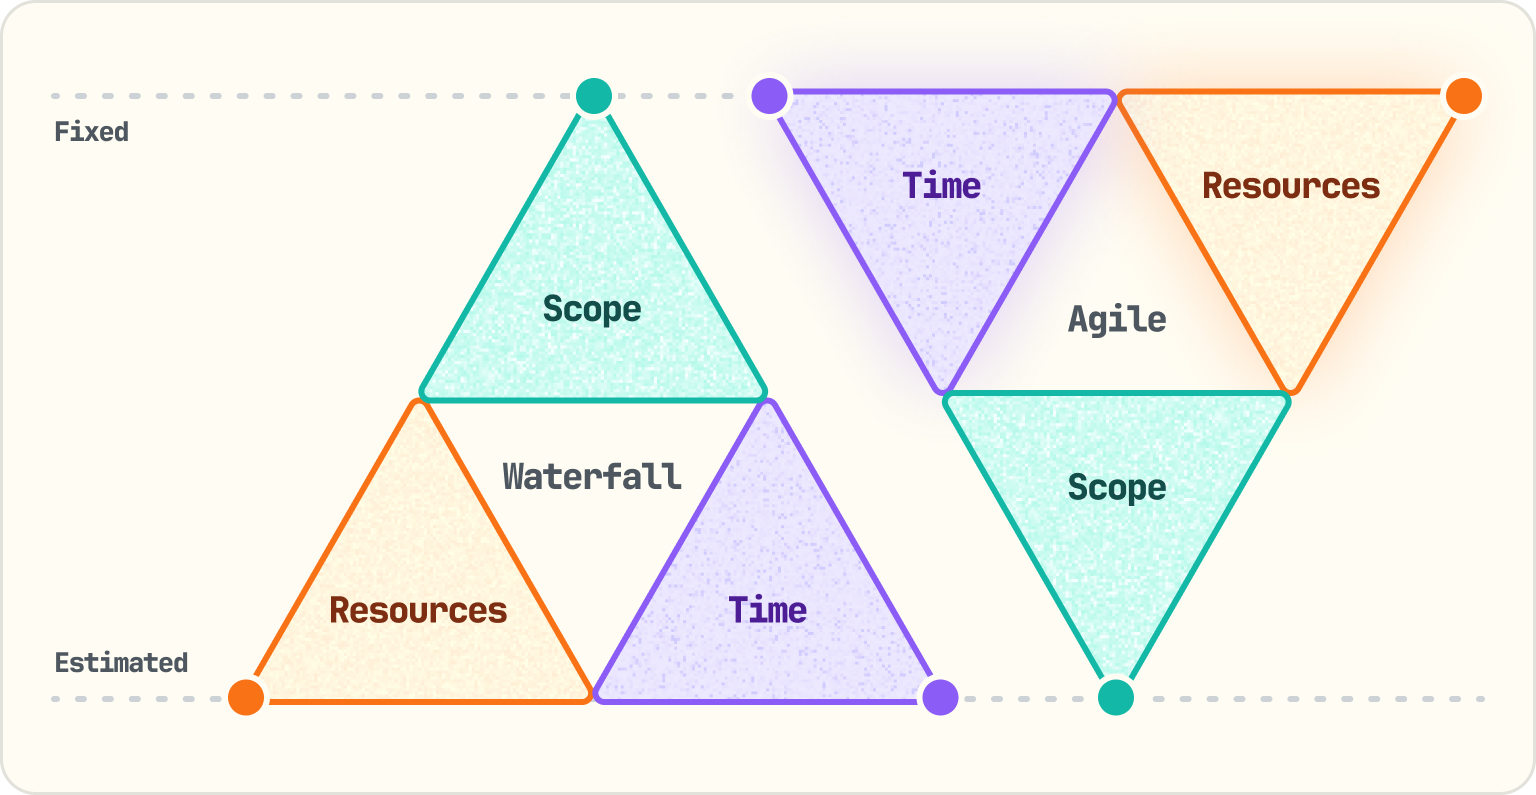
\includegraphics[width=300pt]{Chapter 3/Agile Triangle.png}
    \caption{Project management triangle (Source: own illustration based on Atlassian https://www.atlassian.com/agile/agile-at-scale/agile-iron-triangle)}
\end{figure}
% NOTE DONE:  Mention the triangle:
% https://www.ecosia.org/images?addon=firefox&addonversion=5.1.1&q=agile+vs+traditional+triangle#id=88D37B800865C1E5C05FA187E99967170A4BCFEF 

Scrum also relies on meaningful meetings, like the daily stand-up, where the whole developer team
comes together discussing what the individual members did the previous day, what they are going to
do today and whether there are any blockers. This way, everyone is involved and can help where help
is needed. \vglcite[9]{schwaberScrumGuideDefinitive2020}

\begin{figure}[H]
    \centering
    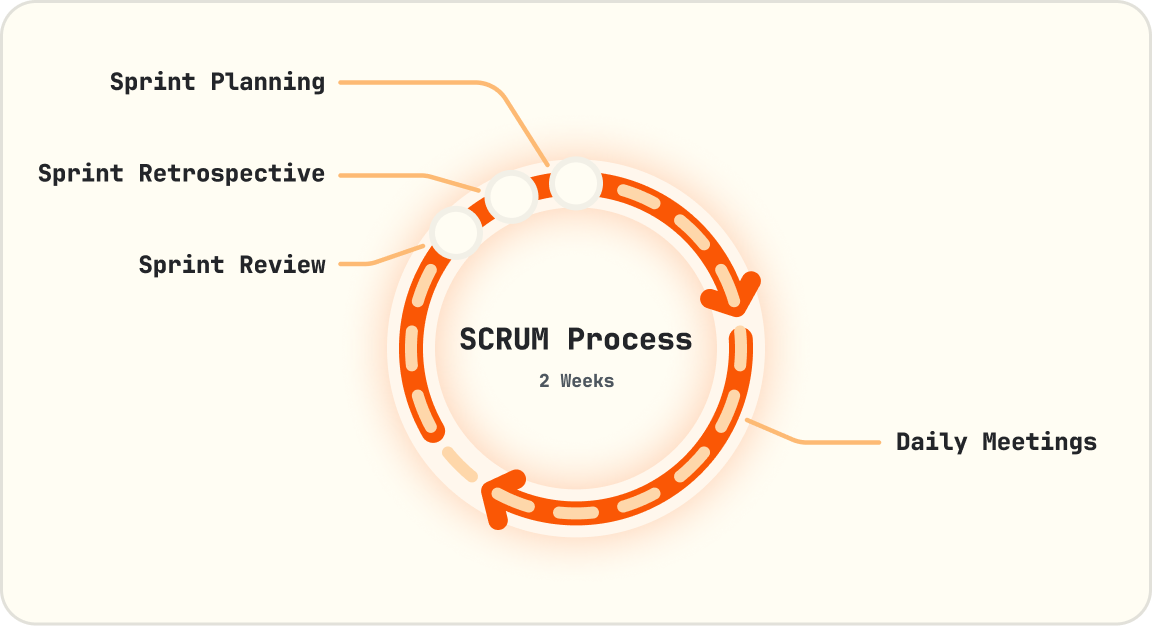
\includegraphics[width=300pt]{Chapter 3/Scrum Process.png}
    \caption{Scrum process (Source: own illustration based on Atlassian https://www.atlassian.com/de/agile/scrum/sprints)}
\end{figure}
% NOTE DONE: Add graphics of scrum process

That brings the design of web projects a lot closer to the desired outcome. Iteratively building the
solution allows for continuous adaptation to feedback and change. Moreover, it ensures a fitting and
working product at all times. However, where does design fit in all of this? This is where Lean UX
comes in. 

\subsubsection{Lean UX}
% For example Dual Track Agile. Then explain why Lean UX has the best things for my
% ways since small teams work well with it to be integrated, so also design can be as iterative as
% development. Especially working well in small teams. Maybe mention Dual-Track Agile and also the
% risk of it creating silos again.

% Hmm lets skip dual track agile and not mention that much about it. It is however also mentioned in
% Lean UX so lets see how I can integrate that.
In their book \textit{Lean UX}, Jeff Gothelf and Josh Seiden describe how Lean UX is a way of
integrating UX/UI Design into Agile software projects. They build on the core values of the Agile
Manifesto and prove that design can be as iterative as development.

The main idea is to work in small, cross-functional teams that build a shared understanding of the
product, the customers and the business goals. These multidisciplinary teams work closely together
minimizing the need for long handoffs. Also, through diverse perspectives, the potential to create
better solutions is maximized. 
\vglcite[24, 26]{gothelfLeanUXProduktentwicklung2016}

So, how does this process actually look like? The process is broken down into four main parts:

% NOTE: Maybe add a graphic of the Lean UX process

\textbf{Outcomes, Assumptions, Hypotheses} \\ % (Lean UX page 38)
Designers and non-designers get together to formulate assumptions, guided by high quality problem
statements. These assumptions contain statements about what the team believes might be true for the
product given the constraints of the problem statement. Then, assumptions are turned into hypotheses
that can be designed and tested by their expected outcomes. After prioritizing the hypotheses by
looking at their value and risk, the team can start designing.
\vglcite[38, 62]{gothelfLeanUXProduktentwicklung2016}

\textbf{Design it} \\
Designers call informal collaborative design meetings or so-called Design Studios, where the whole
team does brainstorming and sketching. Another idea mentioned are one-to-one, designer-dev sessions.
In these meetings everyone gets to come up with ideas and sketches of low-fidelity. That way the
designers have a great pool of diverse ideas to work with.
\vglcite[63,67]{gothelfLeanUXProduktentwicklung2016} 

\textbf{Create an MVP} \\
Creating an Minimal Viable Product (MVP) has the goal of learning as much about the target audience
as possible in the least amount of time. With the hypotheses and the designs in hand an MVP can be
created by asking a question like \textit{What is the least amount of work we can do to achieve
    this?}. By doing this, no resources are wasted to do something which brings no or little value and
the team can implement features quickly and informed.
\vglcite[92, 93]{gothelfLeanUXProduktentwicklung2016}

\textbf{Research \& Learning} \\
With the MVP in place, testing can begin to validate assumptions and hypotheses. With collaborative
research techniques or customer feedback, again every team member gets in contact with this aspect
of building a product, adding to the shared understanding of it. These learnings feed the next cycle
of this process. \vglcite[110, 113]{gothelfLeanUXProduktentwicklung2016} \\

It can be seen that this process includes several fun and innovative methods that push collaboration
even further. The Design Studio for instance, brings the whole team together to sketch out ideas for
specific problems. Although these sessions are led by a designer, everyone contributes and is part
of the design process. \vglcite[68,69]{gothelfLeanUXProduktentwicklung2016}

Another proposed method is called collaborative design, where a minimum of two members come together
to work on a specific problem and sketch ideas rather informally. Often these informal discussions
result in the best and most creative solutions.
\vglcite[66]{gothelfLeanUXProduktentwicklung2016}

These practices all lead to more shared knowledge and understanding and help developers be part of
the design process and vice versa. The whole team moves from blindly implementing features to seeing
the holistic picture and focusing on solving real-world problems - the team culture is positively
different.

As suggested by the authors, this process can also be integrated into the Scrum framework. This
seems to be the best way of introducing Lean UX principles to existing teams, since Scrum is by far
the most used Agile framework.
\vglcite[13]{kpmgAgileTransformationAgile2019}
% NOTE: is there more to say about this? Like how do they suggest it to be integrated? (Lean UX page
% 140) Naaahhh

\newpage
\subsection{Conclusion}
% To make great User Interfaces and User Experiences, it is not enough for designers to do their job
% and developers implementing designs. All disciplines need to work towards that goal and understand
% why something is done and why it is that way. Everyone should be able to understand why the stop
% button of their timer app is that big and at the top right, instead of mini and at the bottom
% left.

As seen in this chapter, the way a project is managed and what \textit{rules} the team follows, have 
a huge impact on the outcome. While the traditional Waterfall model can work for projects with a
fixed scope, it may not be the way to go for design focused web projects as they are usually prone
to change while in development.

To make great User Interfaces and User Experiences, it is crucial that all disciplines work closely
together and understand the \textit{why} behind decisions. Agile methods like Lean UX and the
combination with Scrum seem to be one of the best ways to achieve this change in culture.
Breaking down silos and integrating engineers into the design process will lead to better, more
technically feasible, and developer friendly designs. 

Promoting more informal meetings like collaborative design sessions can also help designers and
developers to understand requirements of each others work better. 


\newpage
\section{User Research}
After looking at the basics of web design and how projects can be structured in an iterative and
collaborative way, we have discovered there are practices that can help to bring design and code
closer together. In this chapter, we take a closer look at how designers and developers work
together in the real world. 

This was done by conducting a qualitative survey and doing interviews with professionals. The shared
goal was to find common pain points, practical solutions and best practices. Also, by inviting both
disciplines to participate and tailoring the questions to their respective fields, I aimed to get a
holistic view of how they percieve each other's work and how well their expectations to each other
align.

% Even when working iteratively or agile there are still handoffs between design and development.
% This is inevitable and has to be done right.

\newpage
\subsection{Survey}

\subsubsection{Goal of the Survey}
The goal of this qualitative survey was to gather in-depth data about designer-developer
collaboration patterns and identify key friction points in their workflows.

\subsubsection{Survey Design}
Although the survey was designed to be answered by both designers and developers, the questions were
tailored to their fields. After an initial question about their role, the survey branched into two
paths. One for designers and one for developers. While the structure and order of the questions
remained similar, the wording and focus of some was slightly adjusted. The thought behind that was
to make it easy for both parties to answer, while being able to compare and align the responses
later on.

Examples of questions include: % NOTE DONE: show them in a better way than a table... Nah Table is ok
\begin{center}
    \begin{tabular}{|m{7.5cm}|m{7.5cm}|}
        \hline
        \textbf{Designer Question}                                                                         & \textbf{Developer Question}                                                                                \\
        \hline
        How would you rate your understanding of web development?                                          & How comfortable are you working with design tools like Figma?                                              \\
        \hline
        What do you think were the main reasons for these discrepancies between design and implementation? & What issues do you commonly face with design handoffs and implementing designs?                            \\
        \hline
        When making a new version [\dots], how do you communicate these changes to the developers?         & When a component needs to be changed, [\dots] how do you expect the designer to communicate these changes? \\
        \hline
    \end{tabular}
\end{center}

Formulating the questions in this way allowed for seeing if there are any discrepancies in the
workflow and how expectations align. The majority of questions were multiple choice, with some
open-ended ones to allow for some more reflective answers. Also, the survey included custom graphics
and a hint of humor to make it more engaging.
% NOTE DONE: show the graphics specially made for the survey

As the survey was designed to reach both beginners and experienced professionals, the survey was
distributed to a wide range of channels:
\begin{itemize}
    \item Two small web development companies with a focus on design
    \item A list of Design and Software Development students at FH Joanneum
    \item LinkedIn connections
    \item Personal designer and developer contacts
\end{itemize}

\subsubsection{Presentation of Survey Results}
Over a duration of 30 days, 31 people responded to the survey. 13 of which considered themselves
primarily as designers, 9 as developers and 9 were not in the target group. While the sample size is
small, the results are qualitative and provide valuable insights and perspectives.

The majority of designers have not yet had as many years of professional experience as the
developers.
% NOTE DONE: Show some numbers here, bar graphs with two bars (one for designer one for developer could
% be suitable here)

The survey supported online claims of Figma being the most popular design tool. 85\% of designers
said they use Figma for designing interfaces. Tools like Photoshop are still used by 25\% as
secondary tools.

\textbf{Knowledge of the other discipline:}\\
When asked about their understanding of the other discipline, the majority of designers rated their
web development knowledge at 3/5 stars, knowing the basics of HTML, CSS and JavaScript. 2 of
them even rated it as "5/5 stars - Honestly could do the developers job :)". Also Developers seem to
know their way around design tools like Figma with 75\% rating their comfort level as 3/5 or higher.
Responses suggest that while there is a general understanding of the other disciplines tools, there
is room for improvement.

\textbf{Discrepancies between Design and Implementation:}\\
81\% of designers said they have experienced discrepancies between design and implementation. The
most common reasons being time constraints, misinterpretation by developers and "Special cases like
complex animations, Popups, Microinteractions". When asked about the main issues with design
handoffs, developers claimed that "Too few designed states (missing hover, focus, \dots)" and
the unclarity of responsive layouts were the most common. Noteworthy is also that devs think complex
components as well as animations, popups or modals are often not well enough specified or
documented. Furthermore, designs not having a component-based approach seem to be a problem, despite
over 80\% of designers claiming they work with such an approach.
These results suggest that there is a common ground for persisting issues. While designers seem to
be aware of component-based design, there may be a misalignment in how it is understood between
disciplines.
% NOTE: In discussion mention that maybe the designers should learn component based design a little
% better or that they should learn how to structure them better

\textbf{Communication:}\\
Despite none of the engineers thinking that "lack of communication with designers" is a re-occurring
issue, some designers state that "more time together with developer[s] and clear communication"
would be beneficial for the workflow.

Regarding practices that have improved the designer-developer collaboration, the most frequent
mentioned factors were proper documentation, design systems, well-structured components and early
involvement of developers. One developer noted that best results were achieved when the disciplines
tried to work out solutions together:
"Implementing a collaborative approach early on in projects: Continuous check-ins with designers and
developers to find the best solution within the given target, budget, and timeline."
% NOTE DONE: Add Quote here

\textbf{Bad and Good Practices:}\\
Respondents identified several specific bad practices that they would like to see less of in the
future. Here, the most commonly named was that there are too many different components and variants
where it is not needed, with one dev recognizing that maybe designers and developers have a
different understanding of what a component is: "Having similar components in thousands of variants
is the default mode in design tools, while in development having few components with a few variants
is the default". Also "inconsistency throughout repeating patterns" were mentioned as a common
practice as well as not using the already designed or developed components. These results shows
again that a diverging understanding of components may be present and that design systems are not
yet used to their full potential.

On the other hand, helpful practices mentioned by the engineers include using clearly defined design
tokens, fonts and colors consistently as well as defining edge-case behaviours and annotating
components. \\

Building on these findings, the next section discusses the underlying causes and possible solutions
to these problems.

\subsubsection{Discussion \& Conclusion}
% Points to discuss
% - Misunderstanding of components: Designers as well as developers often find themselves asking "Should
%   this be a new component or a variant of an existing one? Or is this not a component after all?".
%   Even in the coding world there are different best practices how to structure components. So, it
%   probably is best to ask the team and agree on some basic guidelines. The basic rule of thumb is
%   if a part of a design is used more than once, it should be a component. Also maybe design tools
%   somehow encourage the craetion of too many components as it is very easy to create a component
%   in Figma. Variants are also very powerful, but should only be used to group together different
%   styles of the same component. This would also lead to a closer design and code parity, since in
%   code this is handled very similarly. (<Button variant="primary" size="large">)

% - Unclear layouts: It seems as though responsive layouts are often not well enough defined. Maybe
%   this is due to the fact that designers are working in a pretty fixed setting. Devs can drag the 
%   browser window easily to see how the design behaves. Also, defined grids are pretty rigid and
%   devs often have a hard time to make them work responsively. A proper definition of how grids
%   behave in different breakpoints could definitely help there => Devs use defined breakpoints,
%   designers should use the same ones to define how the design should behave at those specific
%   breakpoints. Also

% - Time Constraints: It seems as though the time constraints cause a lot of issues. Often
%   documentation and proper definition of edge cases as well as hover, empty states are left out.
%   Maybe prioritizing these aspects more could help. Also maybe doing handoffs more often and in
%   smaller batches like Agile workflows suggest could be helpful, as the developers wouldn't need
%   to wait for the whole design to be finished without proper documentation, but could start
%   working sooner with the parts that are already properly defined. Team working agreements can
%   help with that (Lean UX page 87)

% - Conclusion:
% NOTE: Design and Code Parity: https://designsystemdiaries.com/p/figma-to-code-design-system-parity

A common theme throughout the survey was the misalignment in understanding components. It seems as
if designers and developers are using components a little differently, despite using the same
nomenclature. One of the most frequently asked questions in both disciplines is whether an element
should be a new component, a variant of an existing one, or not a component at all. Although there
are different best practices for structuring components in code, the basic rule of thumb is that if
a part is used more than once, it should be a component. The same could simply be done in design
tools. Variants should be used to group components that use the same properties like layout, state,
size, count or others as Figma suggests. \vglcite{figmaCreatingOrganizingVariants2025}

Generally, establishing some basic guidelines for the team helps to improve design-code parity as it
is possible to have a similar structure in both code and design.
% NOTE DONE: Graphics of design and code parity with like idk <Button variant="primary" size="large"> 

Another frequently mentioned issue was the unclear definition of responsive layouts. While design
tools often work in a rather fixed setting, developers can easily switch their viewport to see how
the design behaves. While grids can already be helpful for both, sometimes sizings are hard to
interpret for developers. When setting up desktop, tablet and mobile grids, it is important to agree
on universal breakpoints used by both groups. Furthermore, defining a number of simple page layouts
with specified maximum and  minimum sizes for certain elements like navigation and content can be
extremely beneficial.
% NOTE: Maybe I can have the spacing shizzle I defined for EA: Nö leider
This way, developers can implement grids more easily without guesswork and even designers benefit as
they can take these defined layout grids as a starting point for page designs. Also, defining tablet
and mobile versions of components directly next to each other can help the developers to quickly
implement and quality check the design.

These suggested practices also improves the consistency of repeating patterns, which was another
problem mentioned in the survey. Design tokens like colors, fonts and spacings also fit into the
same category, although they seem to be managed quite well by designers already.

Lastly, time constraints seem to be the root cause to many smaller details. Tasks that are done late
in the process like documentation, definition of edge cases, empty states or focus states come short
when there is no time left. While teams may not be in control of the deadlines, they can change how
they work together. As described in chapter \ref{Agile Project Management & Lean UX}, working in an
Agile manner with smaller handoffs and much more frequent check-ins can boost the workflow. With
smaller handoffs, it may be possible to prioritise documentation, edge cases and other details more
consistently and earlier in the process.

Lean UX further suggests that teams should create a so-called \textit{Team Working Agreement} to
define how they want to work together. This includes development practices, requirements for design,
working hours and more and is refined with each retrospective meeting.
\vglcite[87, 89]{gothelfLeanUXProduktentwicklung2016} 

This concludes my analysis of the survey results. Although, the sample size is small, the insights
are valuable and serve as a great foundation for the practical part of this thesis. To make sure the
practical work is based on as much research as possible, two additional interviews have been
conducted and summarized in the next chapter.


\newpage
\subsection{Interviews}

\newpage
\section{Solving the Design-To-Code problem}
As the practical part of this thesis, the following chapter describes the process of developing a
solution that aims to solve the Design-To-Code problem. This chapter will outline the goal of this
solution, the ideation and design process, the implementation and how intermediate interviews helped
to shape the final outcome. 

\newpage
\subsection{Developing a Solution}
Creating something that tailors to the struggles of both designers and engineers requires a
carefully considered solution. Guided by a clear vision, an innovative idea, a solid system and a
flexible design language were developed.

\subsubsection{The Vision of High Quality Collaboration}
Before starting to think about solutions, the actual needs of the two parties have to be examined
and a clear vision needs to be set. To do this, the data of the survey done beforehand was used as a
foundation.

\begin{description}
      \item[The need for cross-disciplinary knowledge] - Both designers and developers would benefit
            from more knowledge about the other discipline at places where it matters most. If designers
            knew why using variables for design tokens or why applying Figma Auto-Layout in frames
            matters to devs, they could use these techniques more intentionally. Similarly, if
            developers knew how to use design tools to their advantage, they could skip tedious
            back-and-forth conversations and implement screens with more confidence.
      \item[The need for a shared understanding of components] - Designers should be aware that their
            structure of designs can, to a certain degree, mimic and influence the structure of
            code. As a component based approach is the golden standard of web development and found
            its way into interface design, both parties should share certain principles and best
            practices for components.
      \item[The need for more frequent communication] - Communication is key for frictionless
            collaboration and results in great products. As stated in the book Lean UX, the user experience
            is "created by a team, not an individual user interface designer".
            \directcite[63]{gothelfLeanUXProduktentwicklung2016} As remote working models become more
            popular, this becomes an even bigger challenge.
      \item[The need for common best practices] - Knowing when and why to use which tools and
            techniques would benefit the design handoffs drastically. Even more so, avoiding bad practices
            could save hours of reworking documentation, redoing designs or code implementations.
\end{description}

These four needs should be satisfied by the solution. The following sentence should serve as a
vision for the practical project.

% Something fancy incorporating all the needs specified above
\begin{figure}[H]
      \centering
      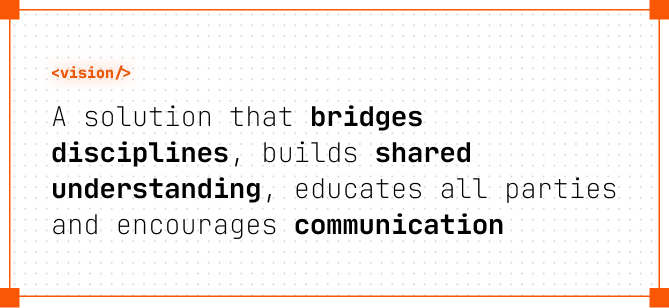
\includegraphics[width=300pt]{Chapter 5/Vision.png}
      \caption{Vision of hight quality collaboration (Source: own illustration)}
\end{figure}

\subsubsection{The Idea of a Shared Interface}
% Saying that the idea of an API is that no matter the platform there is a place that can be
% referred to, to get data, to be informed. Probably could take a page and quickly quote the
% definition of an API

% This concept can be applied to my practical work: A
% centralized place to get helpful tips, how-tos, best practices, communication ideas no matter the
% discipline. The DesignAPI is born: Design Alignment, Principles, Interchange. Being able to refer
% to it more often than once.

In programming realms, there is a widely known and used concept called API. Michael Goodwin
describes it perfectly saying an "API, or application programming interface, is a set of rules or
protocols that enables software applications to communicate with each other to exchange data,
features and functionality." \directcite{michaelgoodwinWhatAPIApplication2024} Upon hearing about a
great software, many devs respond with "Does it have an API?". This is because APIs are a place to
refer and get back to when you need functionality or data. It is a standard.

When it comes to the UI design process and the inter disciplinary collaboration, there is no such
thing as an API. Upon hearing about a great way to structure the design of components, no designer
would reply with "Is there an API for that?". My practical work aims to take the concept of an API
and create a centralized place to get helpful tips, how-tos, best practices and communication ideas
no matter the discipline.

The DesignAPI is born: Design Alignment, Principles, Interchange. It is a place designers as well as
developers can refer and get back to as soon as they need practical knowledge or a quick tip. It
serves as a standard of how design-dev collaboration should be done.

\subsubsection{The System Architecture}
% Explaining what the thing is actually made of: 
% 7 Categories, list each one and what it is about and opportunities for content to fit the needs as
% well: f.e. Figmafication: Opportunity to show devs why using Figma is beneficial.
% 
% For each category there is a set of cards and a set of so-called message templates
% - Consist of a front and a back. Front invites with a title and illustration, back a
%   selection of two to five sections that provide quick info. 

%
%   Explain each section: How to? - Why? - For Devs. Optional: Pro-Tip, Resource

% - Message Templates: To fit modern communication channels like Slack, MS Teams or others, there
%   are templates with Meme character. Again for each category at least one. Each one has a unique
%   purpose and aims to invite frequent playful communication with all team members. 

The DesignAPI starts with six selected categories. Each one covers a unique and challenging topic.

\begin{description}
      \item[States] - Focuses on component states like hover, focus or error that need to be
            designed before implementation. The opportunity for this category is to inform about
            existing states and how structuring them leads to less confusion on both design and
            development side.

      \item[Components] - Focuses on the definition of components, variants and their properties.
            The opportunity for this category is to get closer to a shared understanding of the
            concept of components between the disciplines.

      \item[Styleguide] - Focuses on fonts, colours, spacings or assets. The opportunity for this
            category is to outline the importance of well defined design tokens that can be shared
            between design and code.

      \item[Responsiveness] - Focuses on layouts across screen sizes. The opportunity for this
            category is to communicate best practices that make responsive design a shared
            principle.

      \item[Edge Cases] - Focuses on how general edge cases should be handled in design. The
            opportunity for this category is to reduce overall confusion about how the UI behaves in
            special cases.

      \item[Specials] - Focuses on remaining topics that deserve to be addressed. The opportunity of
            this category is to share little workflow tips for designers.
\end{description}

Each category has its own set of cards and so-called "Message Templates". They are designed to
address the specific opportunities within the category while trying to support the overall vision of
The DesignAPI.

\textbf{Cards}\\
% TODO DONE: write why I chose the card format
Inspired by "Laws of UX" by Jon Yablonski, The DesignAPI features cards that are designed for both
physical and digital use. There is something about this haptic format which makes rigid topics feel
fun and exciting. Like playing cards, the cards of The DesignAPI have a front and a back. The front
invites with a title and illustration and displays its category as well as the number of cards in
that category.
%%% TODO DONE: Add graphics that's like a blueprint of a card showing what's on every card (like my poster
%%% P-OWL)

\begin{figure}[H]
      \centering
      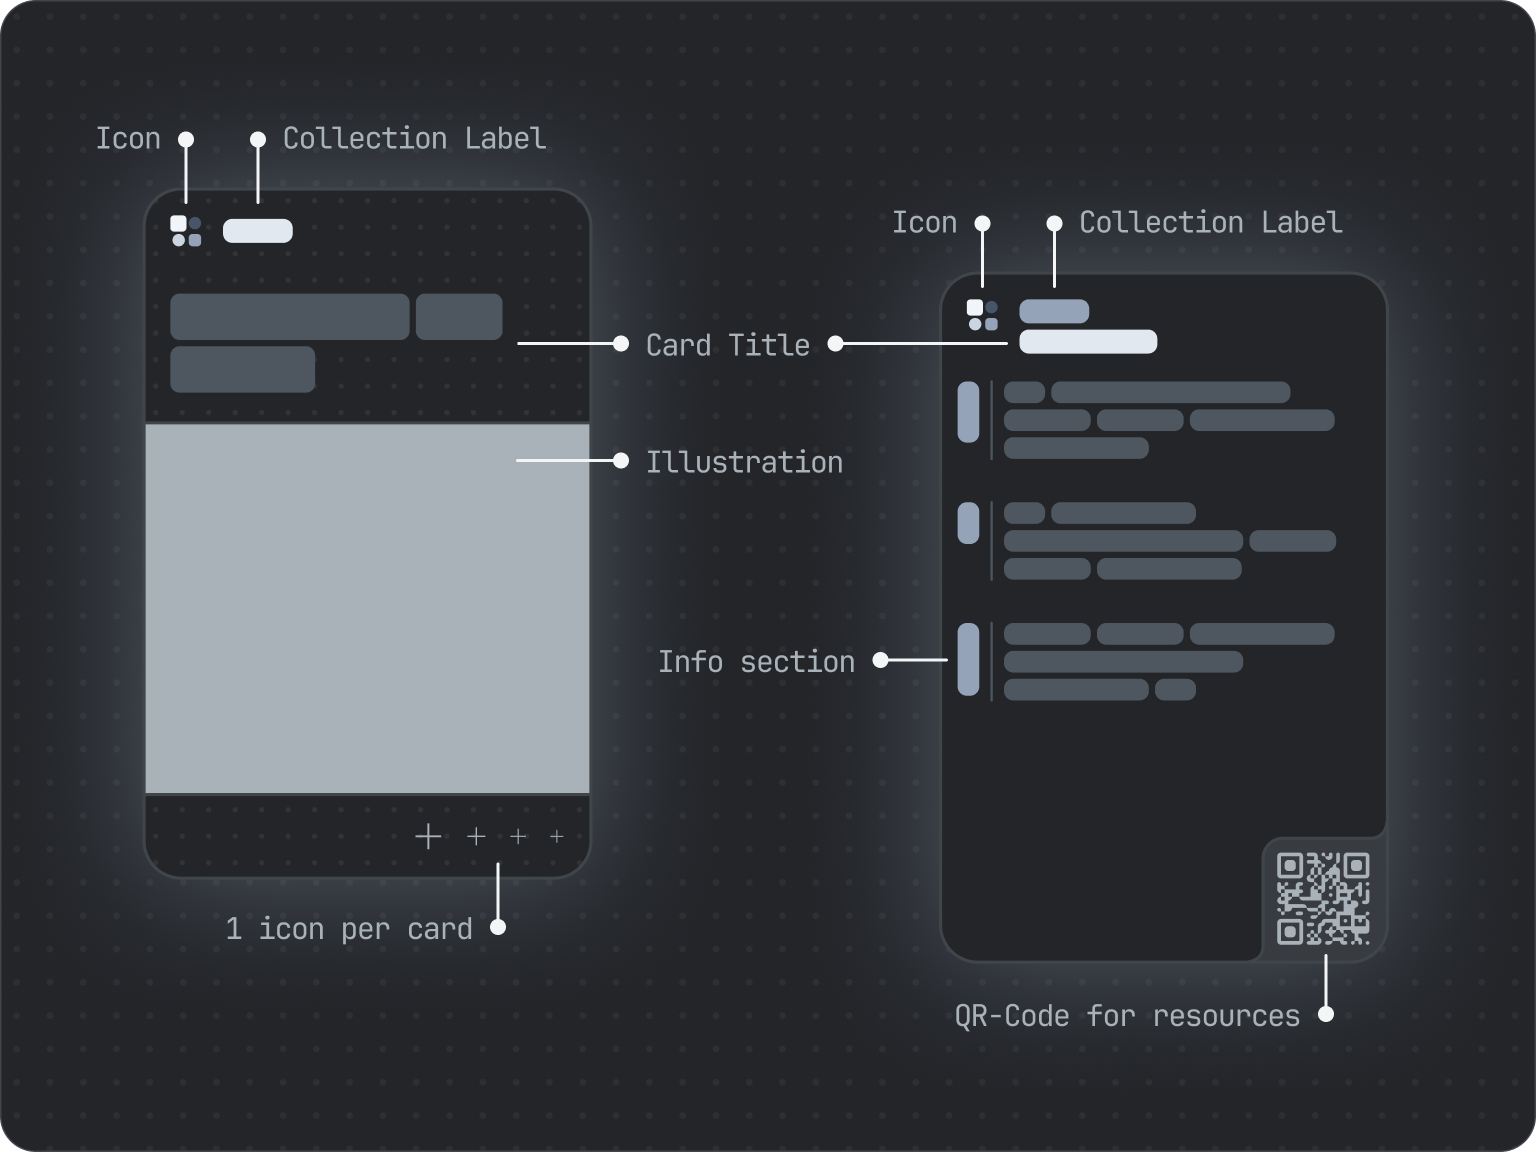
\includegraphics[width=300pt]{Chapter 5/Blueprint card.png}
      \caption{Blueprint of a card (Source: own illustration)}
\end{figure}

The back provides the user with information. It can have two to a maximum of five different sections
of content. Each section has its own purpose:

\begin{description}
      \item[How To?] - Explains what the basic idea or best practice is about and how to
            effectively use it in the everyday workflow.

      \item[Why?] - Outlines the background of the idea and why integrating it is beneficial for
            maximizing the quality of design.

      \item[For Devs] - For most topics, it is important for devs to know what it is about. This
            section brings them into the loop and also provides them with helpful tips. Also,
            designers can get a glimpse of their perspective.

      \item[Pro-Tip] - Often, there are opportunities for another tip on top of the "How To?"-section.
            This is the place for hands-on advice.

      \item[Resource] - Some ideas are communicated best with additional resources such as blog-posts,
            articles or videos. This section highlights that there is a QR-Code to scan to get to the
            external website.
\end{description}

\textbf{Message Templates}\\
% TODO DONE: write that these only make sense in a digital format Nah
The idea of Message Templates is to give team members a gentle nudge to share more design-related
messages with each other. Their purpose is not to replace existing communication, but to enhance it.
It should trigger a change in culture, so that a more frequent, open dialog between designers and
developers takes place.

To fit modern communication channels like Slack or MS Teams, the templates have a fun meme character
to them. This way every message is humorous, as well as informative and helpful.

In contrast to the cards, message templates do not have a rigid structure. As it is a template, they
are meant to be filled with individual content such as screenshots of UI, text or whatever is fits
the context of the template.

\subsubsection{The Design Language}
% Design language decisions
% Design has to be comfortable and inviting, so that users like picking it up and coming back to it often.

% Visual design colorful glass morphism: It should communicate transparency between the disciplines.
% It also adds depth (depth of information). A faint glow shows that it is somehow powerful and worth knowing
% The almost abstract illustrations keeps the content mysterious and interesting.
% (You want to look at the other side to see what it is about => invokes curiosity)

% Fonts and colours. Each category has its own colour shades. This makes it easy to distinct between
% the categories at a glance. 
% The selection of Fonts: 
% - Inter for paragraphs (great and versatile UI Font, default font in Figma
%   => makes designers feel right at home)
% - JetBrains Mono for headers (a font specifically made for developers)
% 
% Taken from both worlds of the spectrum, these fonts were the best choice for this project.

% TODO DONE: Chance for graphics showing different colours and stuff

% Voice and Tone:
% - To make the topic feel more casual all content is written in a rather informal way. 
The design of The DesignAPI must be well considered. It must be comfortable, inviting as well as
exciting, so that users like picking it up and get back to it once they need a tip.

\textbf{Visual Design}\\
% TODO DONE: Add graphics of this glassmorphism style
To meet these goals, The DesignAPI adopts a colourful glass morphism style. The glass-like elements
communicate transparency between disciplines, while layering the elements gives the design depth
much like the richness of information conveyed on the cards.

All unique illustrations are kept in a minimalistic, almost abstract style that makes the viewer
interested in what it is actually about. A faint glow shows that the information is powerful and
worth knowing.

\begin{figure}[H]
      \centering
      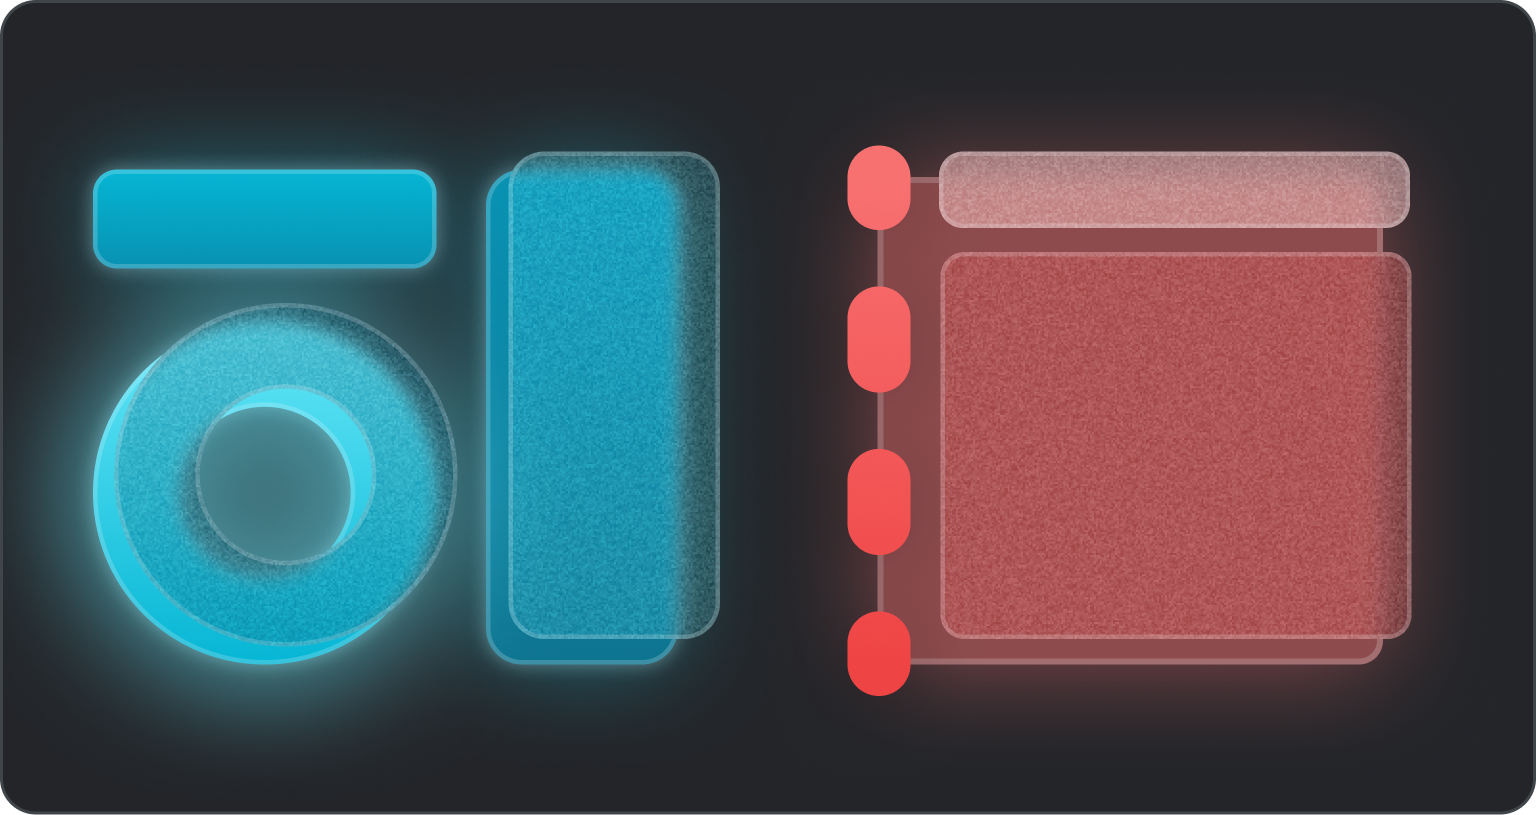
\includegraphics[width=300pt]{Chapter 5/glassmorphism style.png}
      \caption{Visual design: Glass Morphism (Source: own illustration)}
\end{figure}

\textbf{Fonts, Iconography and Colours}\\
Each category has its own primary colour and a number of shades that can be used for icons and
illustrative elements. Furthermore, an individual icon was designed for each category to be able to
easily distinct between them without solely relying on colour.

Moreover, a dark and light mode for all assets using semantic design tokens was integrated, to
make it even more appealing for the target group and to allow for a bit of personalization.
% TODO DONE: Add graphics for colours and category icons

To show the dual nature of The DesignAPI's target audience, the following two typefaces were chosen:
\begin{description}
      \item[Inter] - Used for paragraphs. It is a massively popular typeface mostly used in
            computer interfaces and is the default font in Figma. Using this font, contributes to a
            sense of familiarity for UI designers. \vglcite[]{rasmusanderssonInterTypefaceFamily}

      \item[JetBrains Mono] - Used for headings. It is a typeface made for developers to increase
            readability in code editors. With this font, the goal was to make developers comfortable
            using The DesignAPI. \vglcite[]{jetbrainss.r.o.JetBrainsMonoTypeface}

      \item[Gochi Hand] - Used for author notes. It is an informal font that should resemble a normal
            persons handwriting. This font was used to add useful notes on top of the cards rigid structure
            to add important information and make them feel more lively.
\end{description}

\begin{figure}[H]
      \centering
      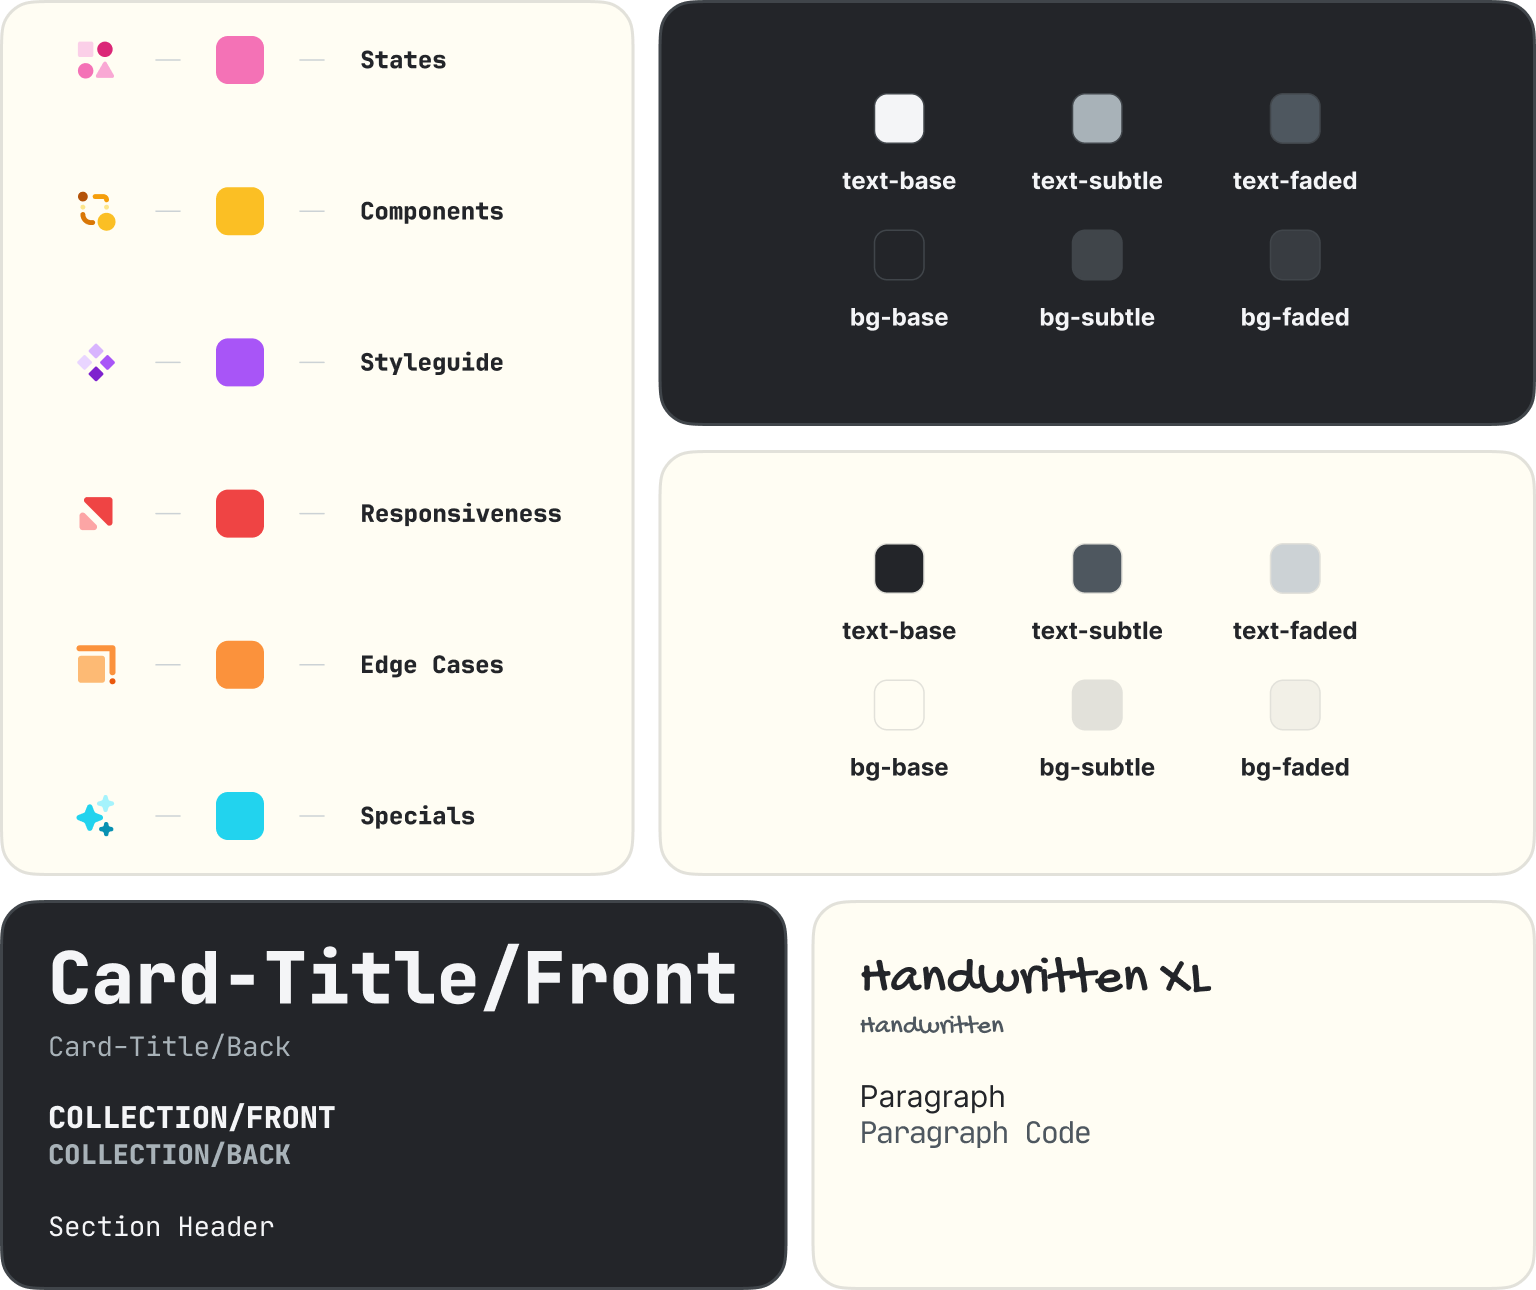
\includegraphics[width=300pt]{Chapter 5/Icons Colors Fonts.png}
      \caption{Fonts, Iconography and Colours (Source: own illustration)}
\end{figure}

% TODO DONE: Add graphics for the fonts in a nice presentation. Maybe all Figma styles

\textbf{Voice and Tone}\\
Reading best practices and guidelines can be exhausting quickly, as their formulation is often very
technical and rigid. The DesignAPI took inspiration from a study examining how different tones of
voice affects the impressions of desirability, trustworthiness and friendliness for a brand.
The study states that "dry industries [...] can benefit from a little conversational language".
\directcite{katemoranImpactToneVoice2024}

Additionally, casual and somewhat enthusiastic language generally performs best as it keeps
desirability and trustworthiness high. \vglcite{katemoranImpactToneVoice2024}
The following figure shows examples of the language used in The DesignAPI.

\begin{figure}[H]
      \centering
      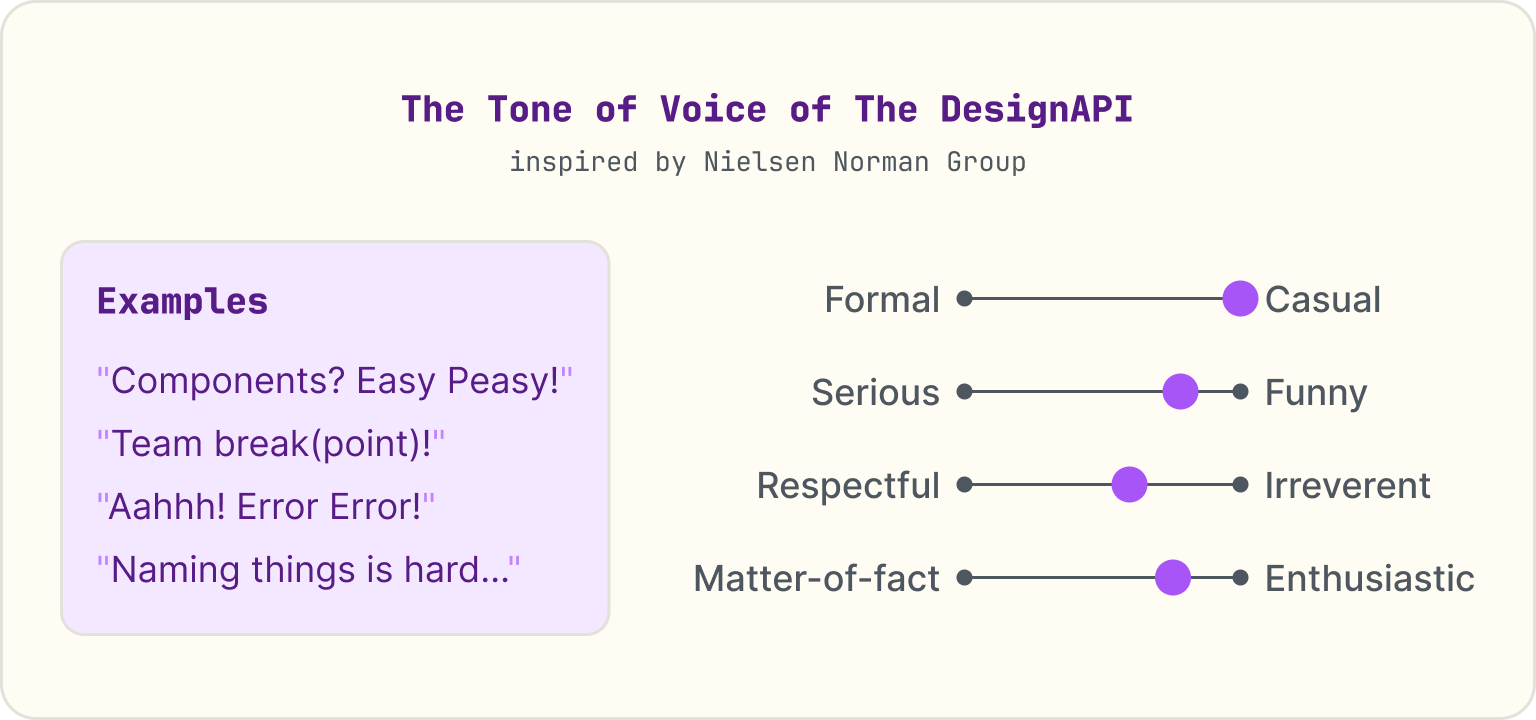
\includegraphics[width=300pt]{Chapter 5/Voice of Tone.png}
      \caption{Voice of Tone (Source: own illustration based on Nielsen Norman Group https://www.nngroup.com/articles/tone-voice-users/)}
\end{figure}
% TODO DONE: Add graphics with these examples and include a graph like this:
% https://media.nngroup.com/media/editor/2024/01/30/example-3.jpg


\newpage
\subsection{Curating and Writing Content}
% Content selection:
% - Mostly from questionnaire and own experience of web UI designer
% - Blog posts from designers and developers
% - Tutorials and articles from Figma itself
% From that a list of topics and their category was selected.
The selection of content and formulating best practices, tips and guidelines was the toughest
challenge of The DesignAPI. It is the core of it all. With the categories in mind, a list of topics
was created from three main sources:

\begin{description}
      \item[Questionnaire and Individual Experiences] - Most topics and content were
            sourced from the analysis of the questionnaire. The real-life experiences, challenges,
            workarounds and already tested best practices were a great foundation. Combined with the
            author's experience in interface design, it was ensured that they could help others.
      \item[Blog posts from known designers and developers] - Articles helped immensely to further
            make sure, the content on the cards is supported by experiences of people who know about
            the struggles of design and code collaboration.
      \item[Tutorials and articles from Figma] - Some cards had to be Figma specific. Figma has a
            dedicated series of articles that show how repeating problems are correctly solved with
            its software. (www.figma.com/best-practices/) A few of the ideas, where included and
            referenced in the content of the cards.
\end{description}


% Writing content:
% For each topic I wrote down everything in the tone of voice specified that popped into my head for
% the necessary sections and included resource references where necessary. After that, I noticed
% that many sections for many cards were simply too long to fit on tiny cards. Which forced me to
% shorten everything => Great idea since it should be short. I chose to use ChatGPT as a way of
% shortening my original content. By prompting it with my original sentences for each card content
% and asking to keep the voice and tone of it just shorter. The answers given were then reworked 
% once more. It really sped up the process, while still staying in full control of the content
% written. This is a small testament of how Large Language Models (LLMs) can be used as a tool to
% enhance efficiency, without losing quality. 
% 

For each topic, the ideas and content in the defined tone of voice were written down, ensuring all
necessary sections were addressed and included resource references where necessary. It was until
after this process, that it became clear many entries exceeded the space on the playing card format.
However, this constraint reminded of the initial goal of keeping information precise and brief.

% TODO: Add graphic that shows this process one more time.
% My original long content => Short content from ChatGPT => finished content with my changes
To refine the content, ChatGPT was used as a tool to help condense the paragraphs. The prompts used,
were crafted to keep the original tone while shortening everything. The generated responses were
then manually revised again to fully support the intended message. This highly iterative approach
both sped up the writing process and showed the potential of Large Language Models (LLMs) to support
content creation workflows. It enhanced efficiency without losing quality or intent.

In chapter 6, all of the cards along with their content are showcased.


\newpage
\subsection{Target Group Interviews}
In order to develop a solution that is truly valuable, it is important to emphasize with the target
group. Directly talking to the people that are part of the process in their day-to-day business
allows exactly for that.

\subsubsection{Goal of the Interviews}
There were two main goals. Firstly, finding more real world experiences and uncovering problems yet
to be found. Secondly, getting immediate feedback on the practical work, so that a quick iteration
can take place. It was a conscious decision to conduct the interviews after having worked on the
solution for some time, since there was already a tangible product to be reviewed by the designer
and developer respectively.

\subsubsection{Participants}
The names as well as the company the participants work for have been anonymized, as this data is not
necessary for the analysis. 
\begin{figure}[H]
    \centering
    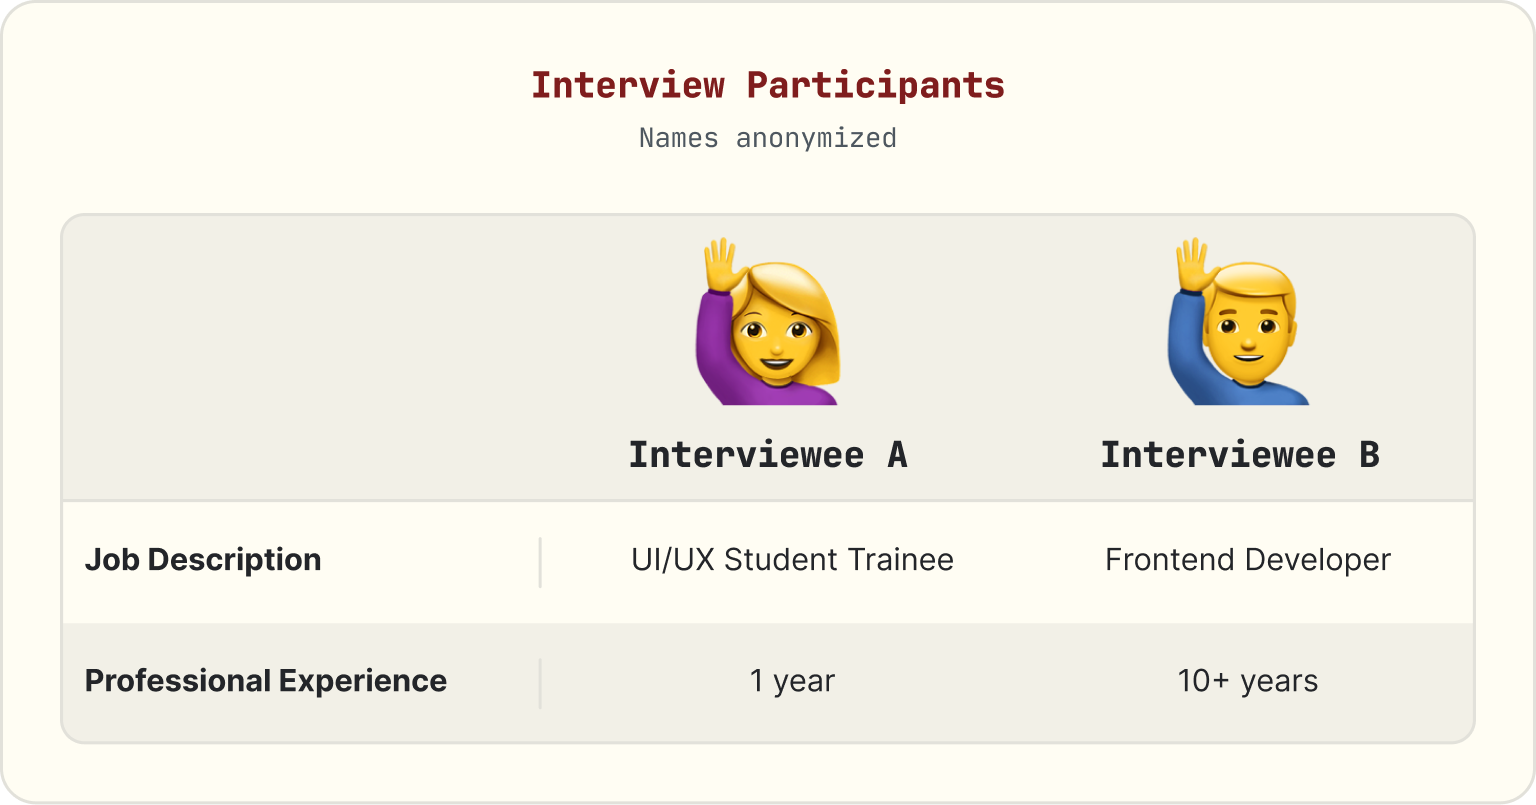
\includegraphics[width=300pt]{Chapter 5/Personas.png}
    \caption{Interview participants (Source: own illustration)}
\end{figure}

%TODO: Quick "Persona" view of those saying changed the names

\subsubsection{Presentation and Conclusion of the Results}
\textbf{Designer Interview}
Interviewee A states that the developers she worked with until now had little to no knowledge of
design tools like Figma. \vglcite[74]{interviewpartnerinaInterview1Gefuehrt2025a} "One of them was
interested, but had only just learnt how to work with it."
\directcite[89]{interviewpartnerinaInterview1Gefuehrt2025a} She thinks this lack of knowledge on
developer side is a serious issue and wishes "that all [developers] know Figma".
\directcite[542]{interviewpartnerinaInterview1Gefuehrt2025a}

Handing off designs is done by manually exporting finished UI components as SVG files and
uploading them to Confluence, a platform developers are comfortable with. She states that "you lose
time if you export everything to Confluence and always have to write a description".
\directcite[680]{interviewpartnerinaInterview1Gefuehrt2025a} Even though documentation is important
this extra step seems unnecessary to her.

Interviewee A has also experienced major discrepancies between design and implementation in one of her
earliest projects. The finished product "looked totally different"
\directcite[452]{interviewpartnerinaInterview1Gefuehrt2025a}, even buttons had completely different
colours. According to her, developers not knowing Figma, budget-cuts and unqualified engineers where
the primary reasons for this \directcite[476, 503]{interviewpartnerinaInterview1Gefuehrt2025a}

\textbf{Developer Interview}
In contrast to the developers interviewee A worked with, interviewee B has worked with Figma for
quite some time. Together with their external UI designer, they built a solid design system for
their product. He notes that while a thought-out structure is not immediately visible and important,
it "helps if there is a certain system over everything, because then you also understand in the code
what the system is and can then map the system in Code".
\directcite[170,173]{interviewpartnerbInterview2Gefuehrt2025a} They also "use the same
design tokens in Figma and in the code". \directcite[146]{interviewpartnerbInterview2Gefuehrt2025a}

His team often notices that designers make decisions, "which [are] in principle a good idea, but
    [the designer] doesn't know what impact this will have on the implementation".
\directcite[281,284]{interviewpartnerbInterview2Gefuehrt2025a} As he and his team try to minimize
unnecessary overload, they evaluate and question designs if they notice high implementation
complexity. They check with the designer if there isn't an easier solution with
a similar value. \vglcite[290,338]{interviewpartnerbInterview2Gefuehrt2025a}

Mentioned practices that speed up development include
\begin{itemize}
    \item easily findable and exportable assets \vglcite[416,434]{interviewpartnerbInterview2Gefuehrt2025a},
    \item unified breakpoints used in both Figma and Code
          \vglcite[863,866]{interviewpartnerbInterview2Gefuehrt2025a} and
    \item responsive components in desktop, tablet and mobile versions as variants next to each
          other in Figma. \vglcite[554-566]{interviewpartnerbInterview2Gefuehrt2025a}
\end{itemize}

\textbf{Conclusion}
The insights of the interviews done allow for further fine tuning and adapting the content of the
practical work. In the next step this tuning process is further elaborated with specific examples.


\newpage
\subsection{Incorporating Feedback}
This chapter explains the process of incorporating the feedback from the target group interviews
into the current progress of The DesignAPI. As many changes have been made, only the most impactful
have been highlighted here.

As Mary mentioned that numerous engineers have never been in contact with Figma, a new category was
added to fill this gap.

\textbf{Figmafication} - Focuses on getting developers familiar with using Figma. The
opportunity for this category is to increase the number of engineers actively
incorporating design tools like Figma into their workflows.

Having unified screen breakpoints and keeping responsive components variants close to each other was
mentioned by Peter as a very helpful practice. This resulted in the following two cards being added
to the collection.
%TODO: Add graphics of the two responsiveness cards 

Lastly, Peters example of a situation where a simple Radio-Button would have done the job perfectly,
but instead the designer came up with a much more complex solution was a powerful story.
Identifying parts of the design that would cost much time to implement, but are valuable in contrast
to parts that don't provide enough value and communicating this early to the designer is important.
(vgl 281-389)
It enables the team to deliver value at parts where it actually matters. This sentiment has been
turned into a card as well as a message template.
%TODO: Add graphics of card and message template.

\begin{figure}[H]
    \centering
    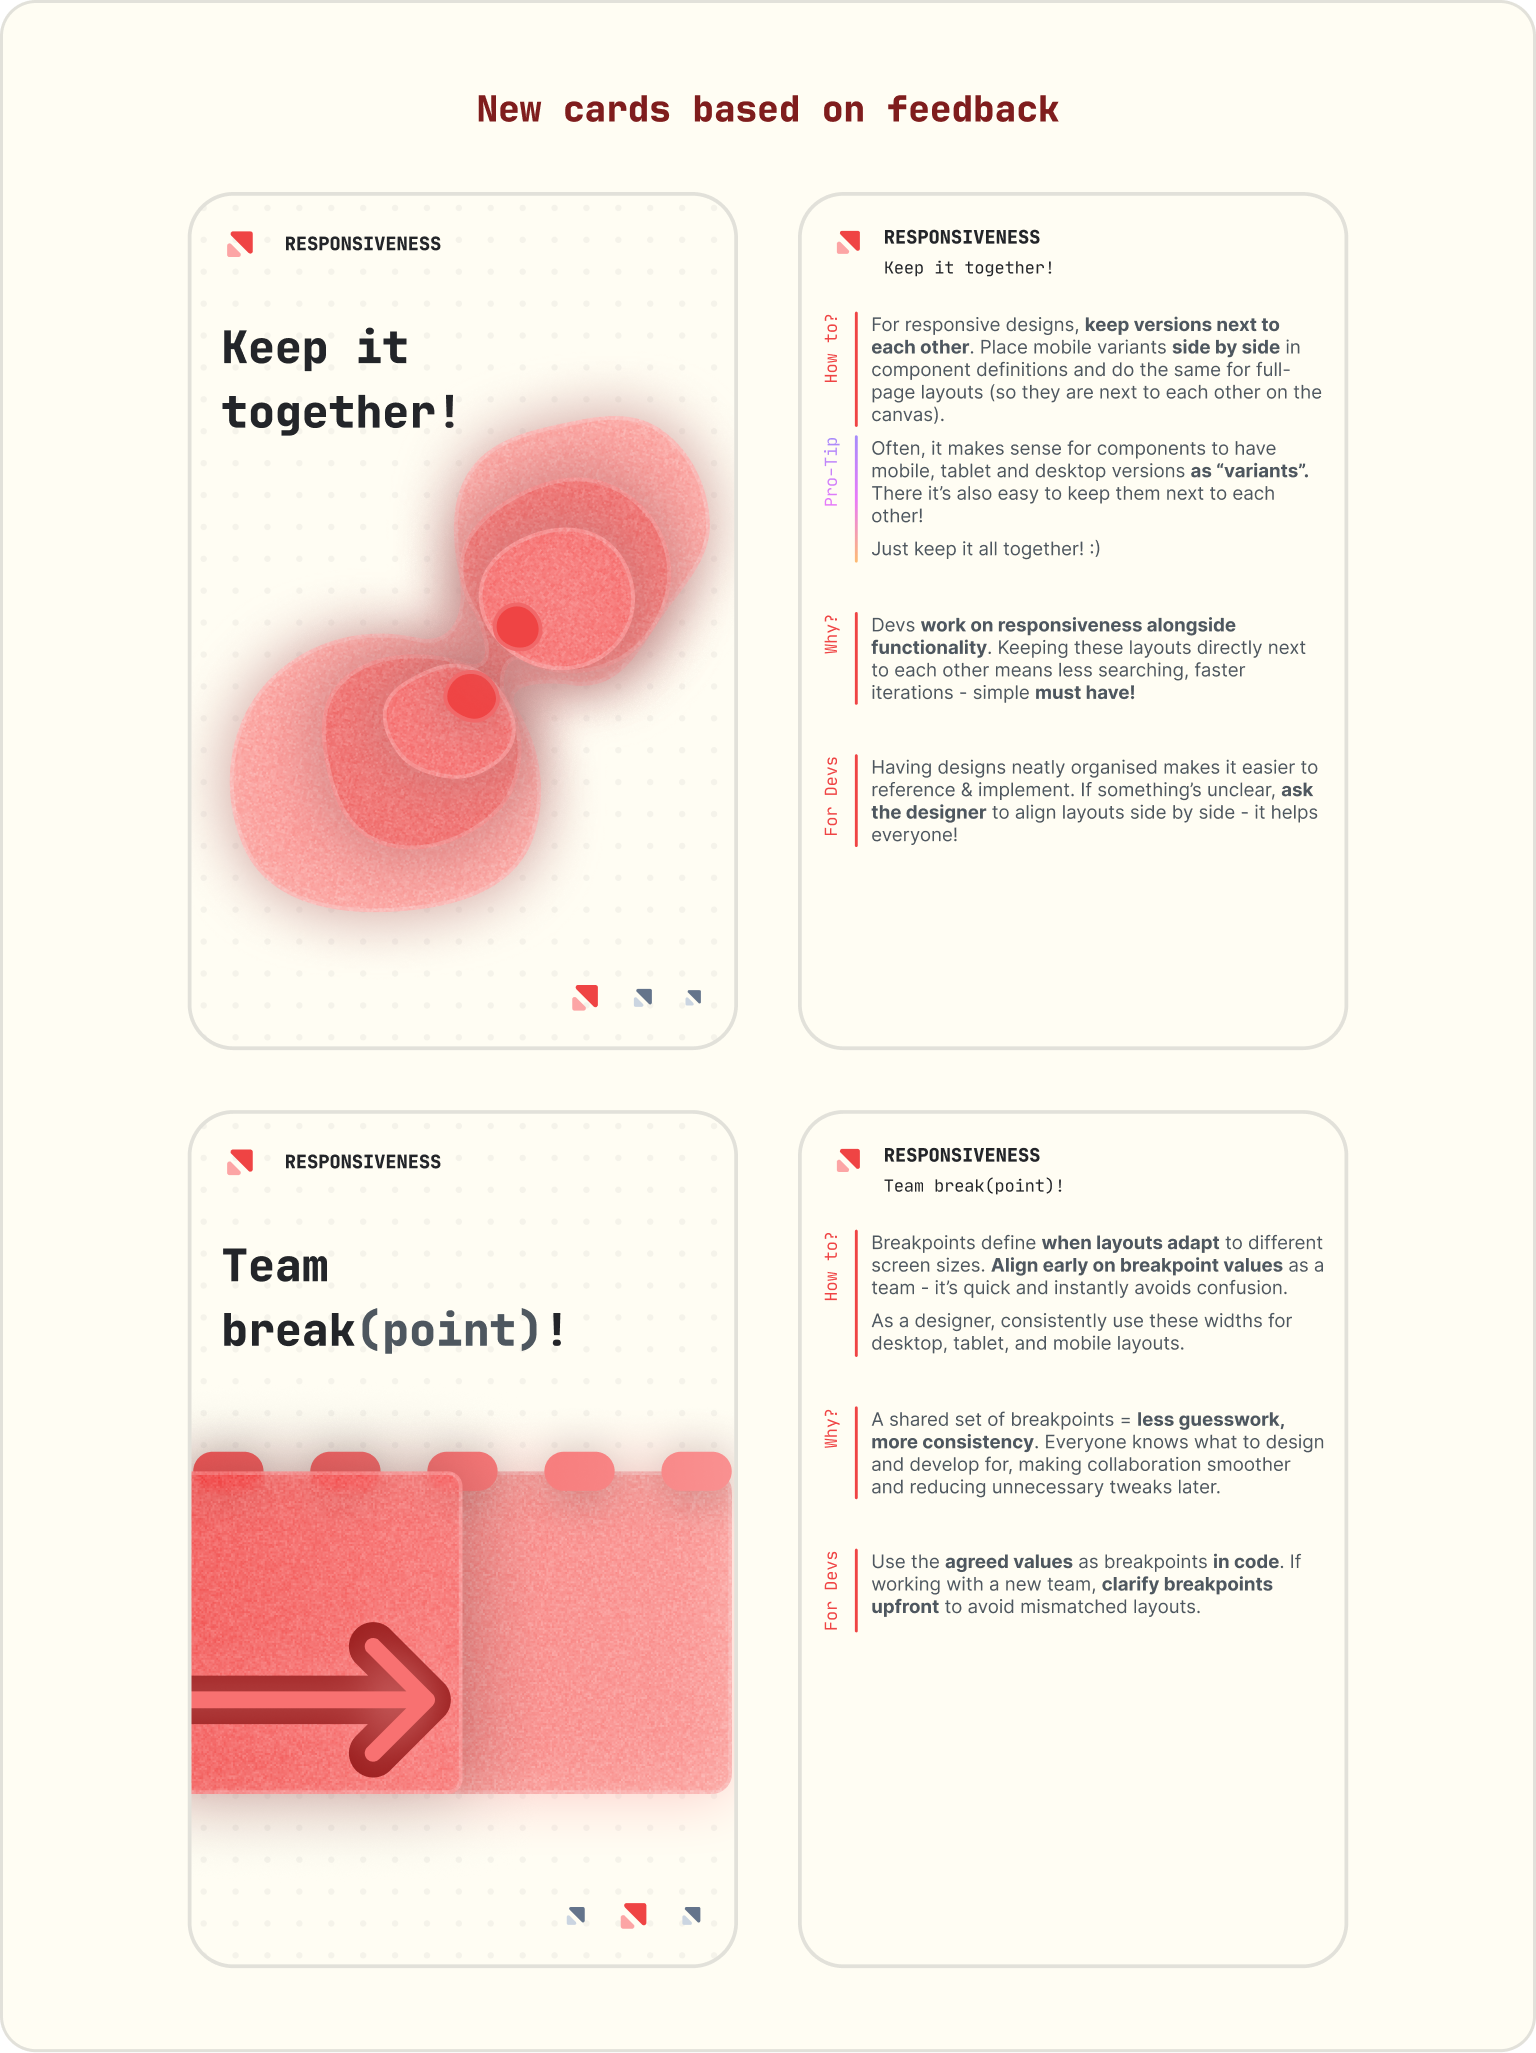
\includegraphics[width=400pt]{Chapter 5/New Cards.png}
    \caption{New cards in the Responsiveness category based on feedback (Source: own illustration)}
\end{figure}

\begin{figure}[H]
    \centering
    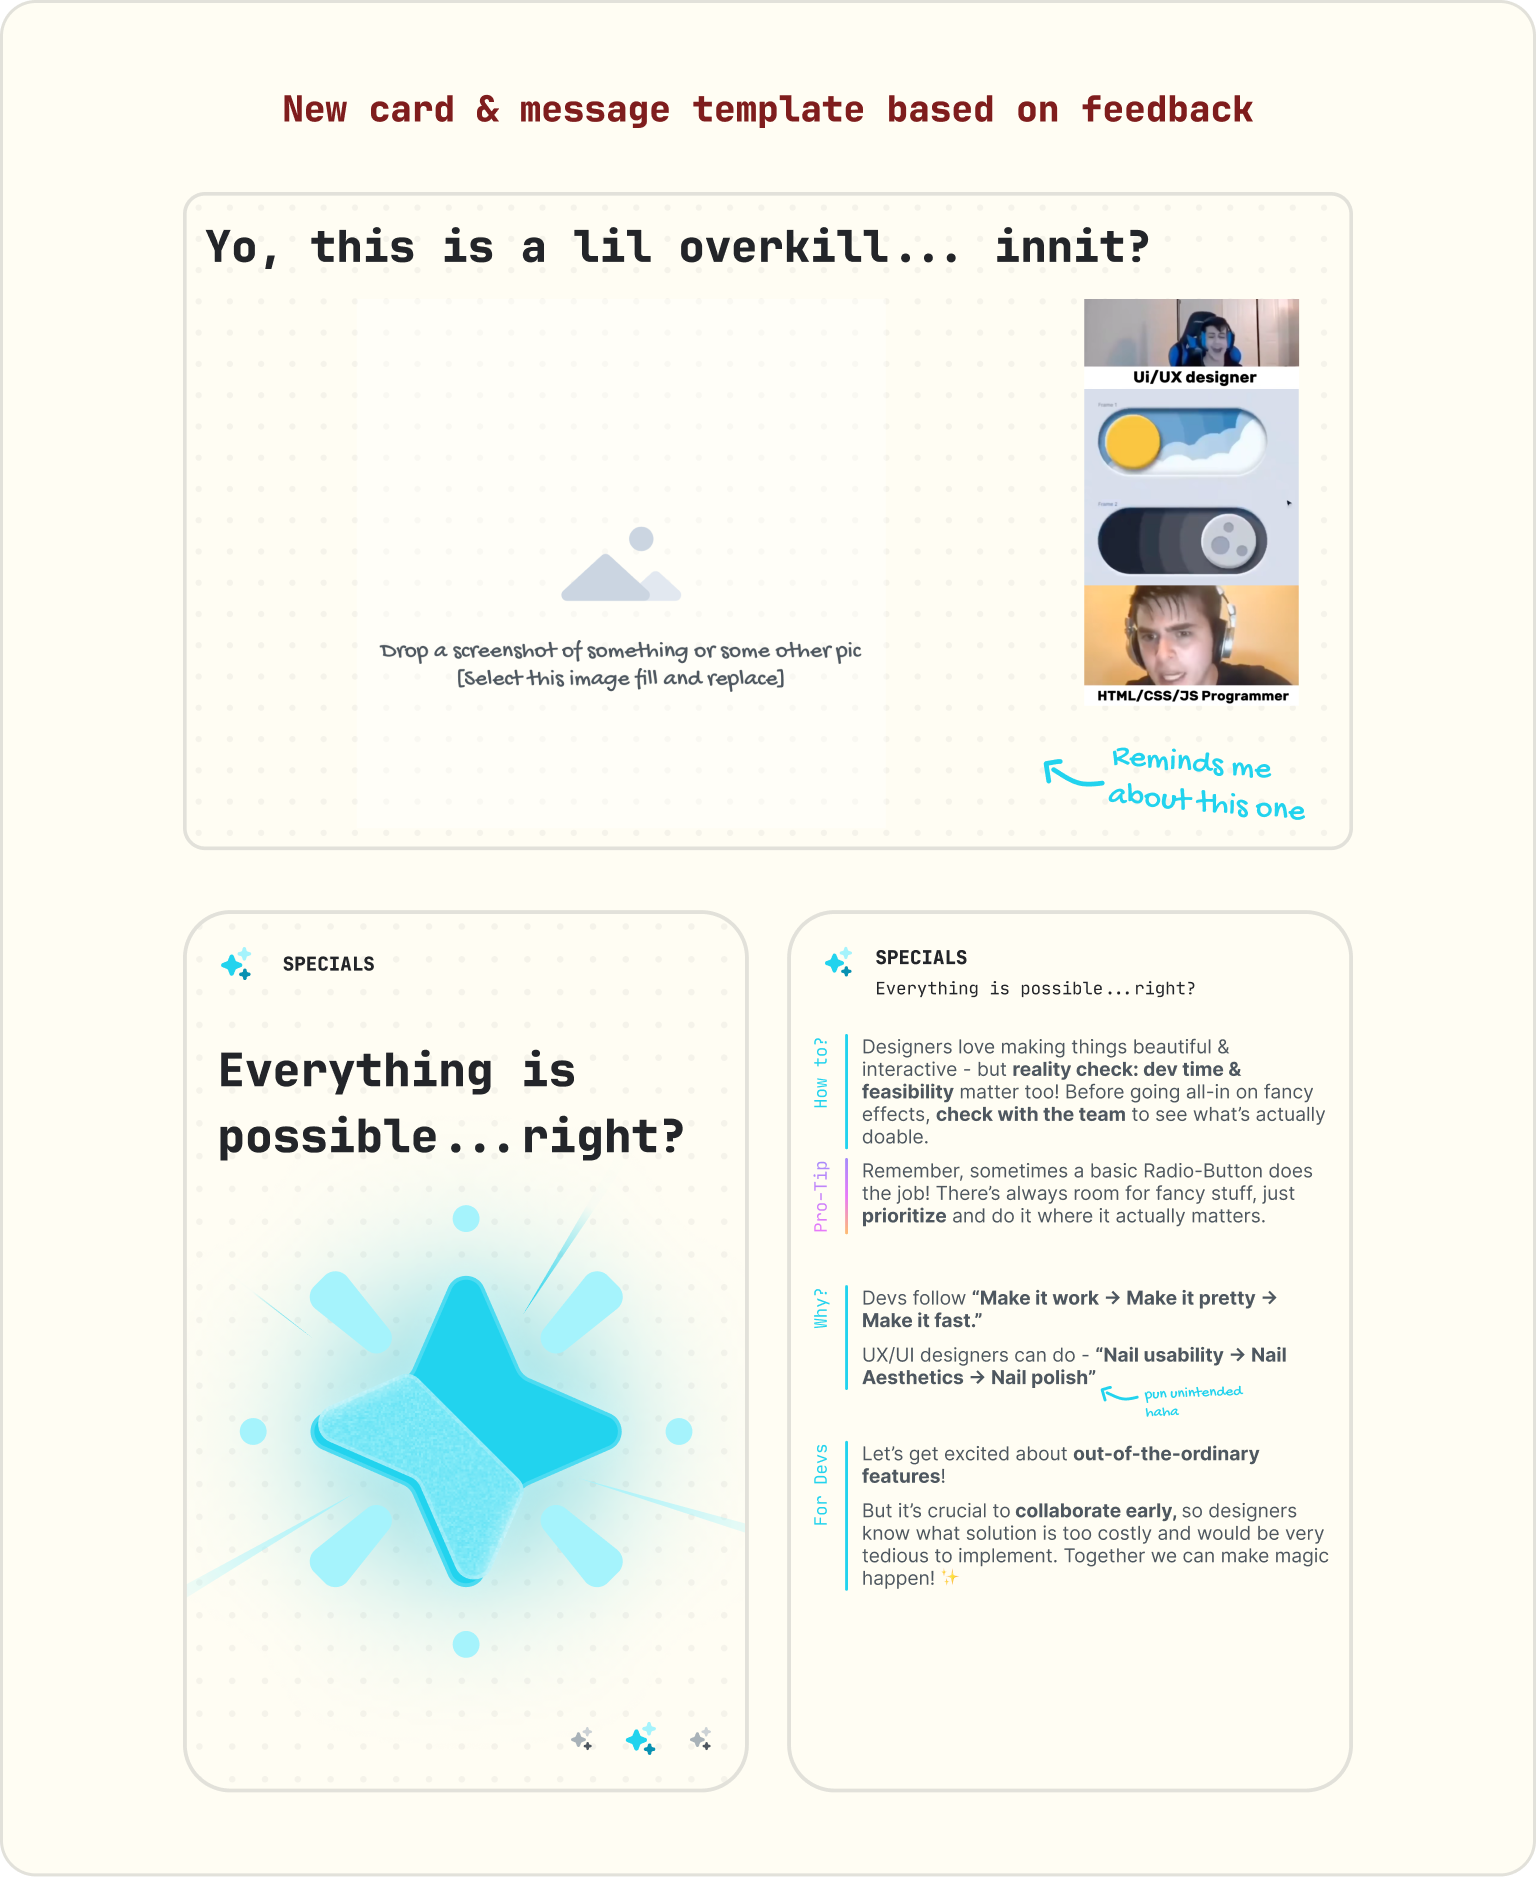
\includegraphics[width=400pt]{Chapter 5/New Card and template.png}
    \caption{New card and message template in the Specials category based on feedback (Source: own illustration)}
\end{figure}


\newpage
\section{The DesignAPI: A Shared Interface Between Design and Code}
With the vision of aligning frontend disciplines, sharing principles and encouraging interchange,
the DesignAPI serves as an innovative shared interface between design and code. Seven categories, 29
cards and 12 message templates. All beautifully designed with content based on research, real
experiences and newly imagined best practices with the goal of harmonizing the two disciplines. This
chapter will present all final assets of the DesignAPI.

\newpage
\subsection{The Cards}
\begin{figure}[H]
    \centering
    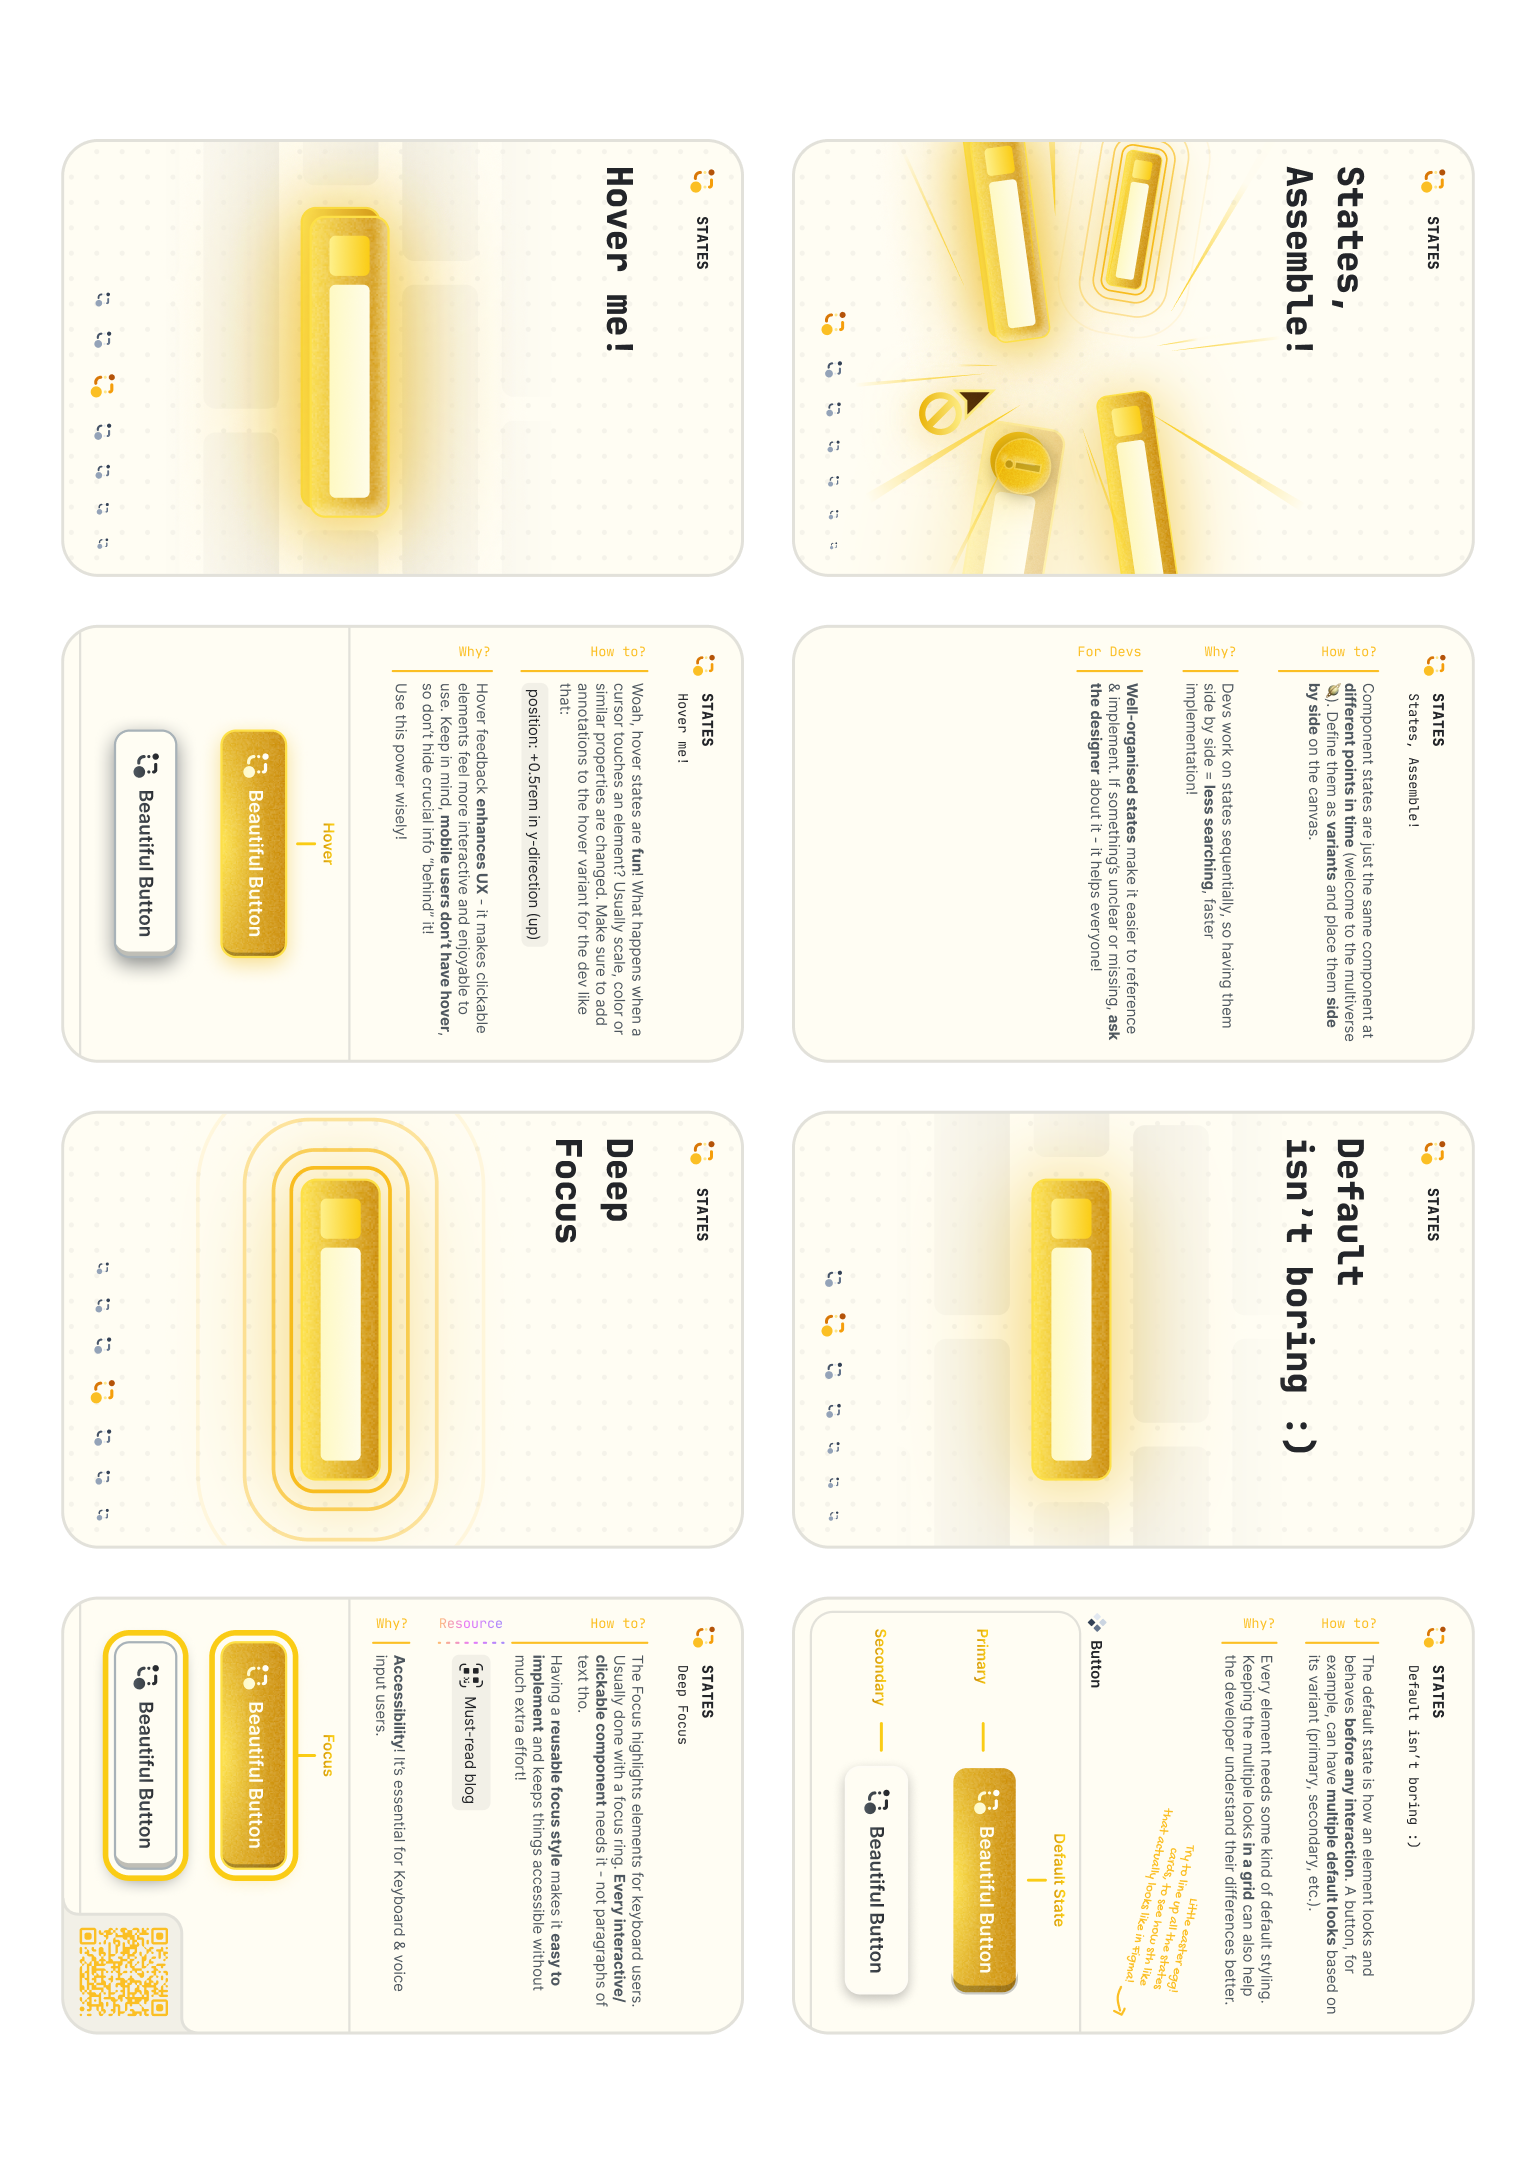
\includegraphics[width=400pt]{Chapter 5/Cards 1.png}
    \caption{The DesignAPI: Cards 1 (Source: own illustration)}
\end{figure}

\begin{figure}[H]
    \centering
    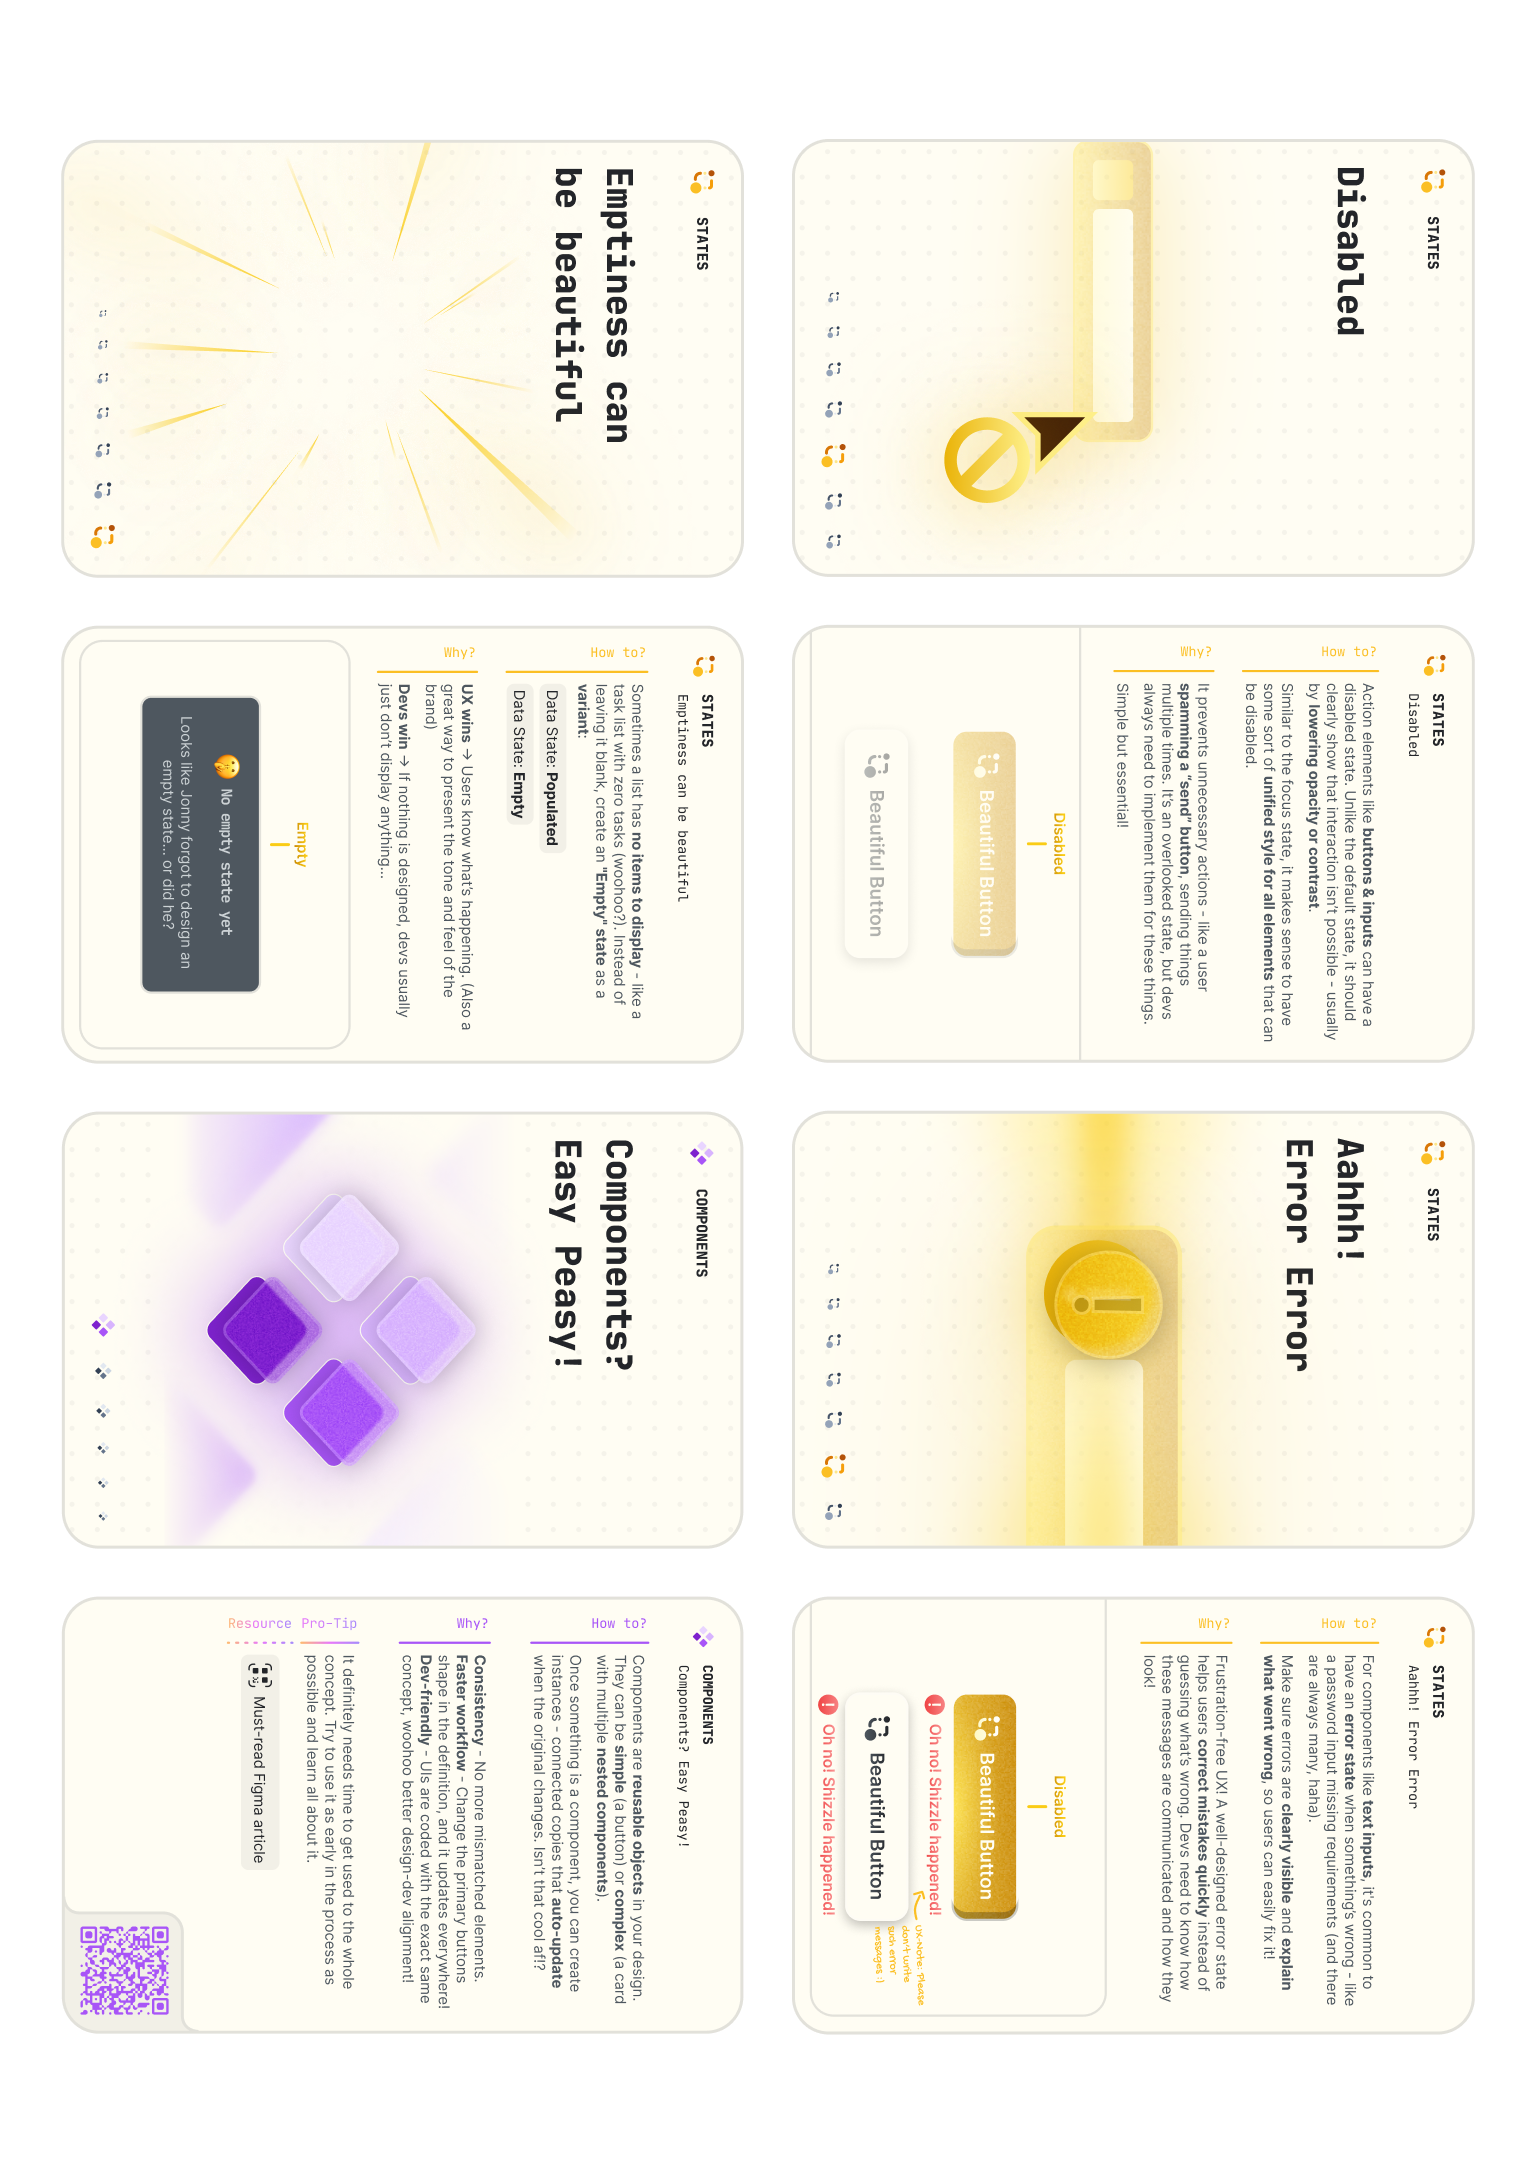
\includegraphics[width=400pt]{Chapter 5/Cards 2.png}
    \caption{The DesignAPI: Cards 2 (Source: own illustration)}
\end{figure}

\begin{figure}[H]
    \centering
    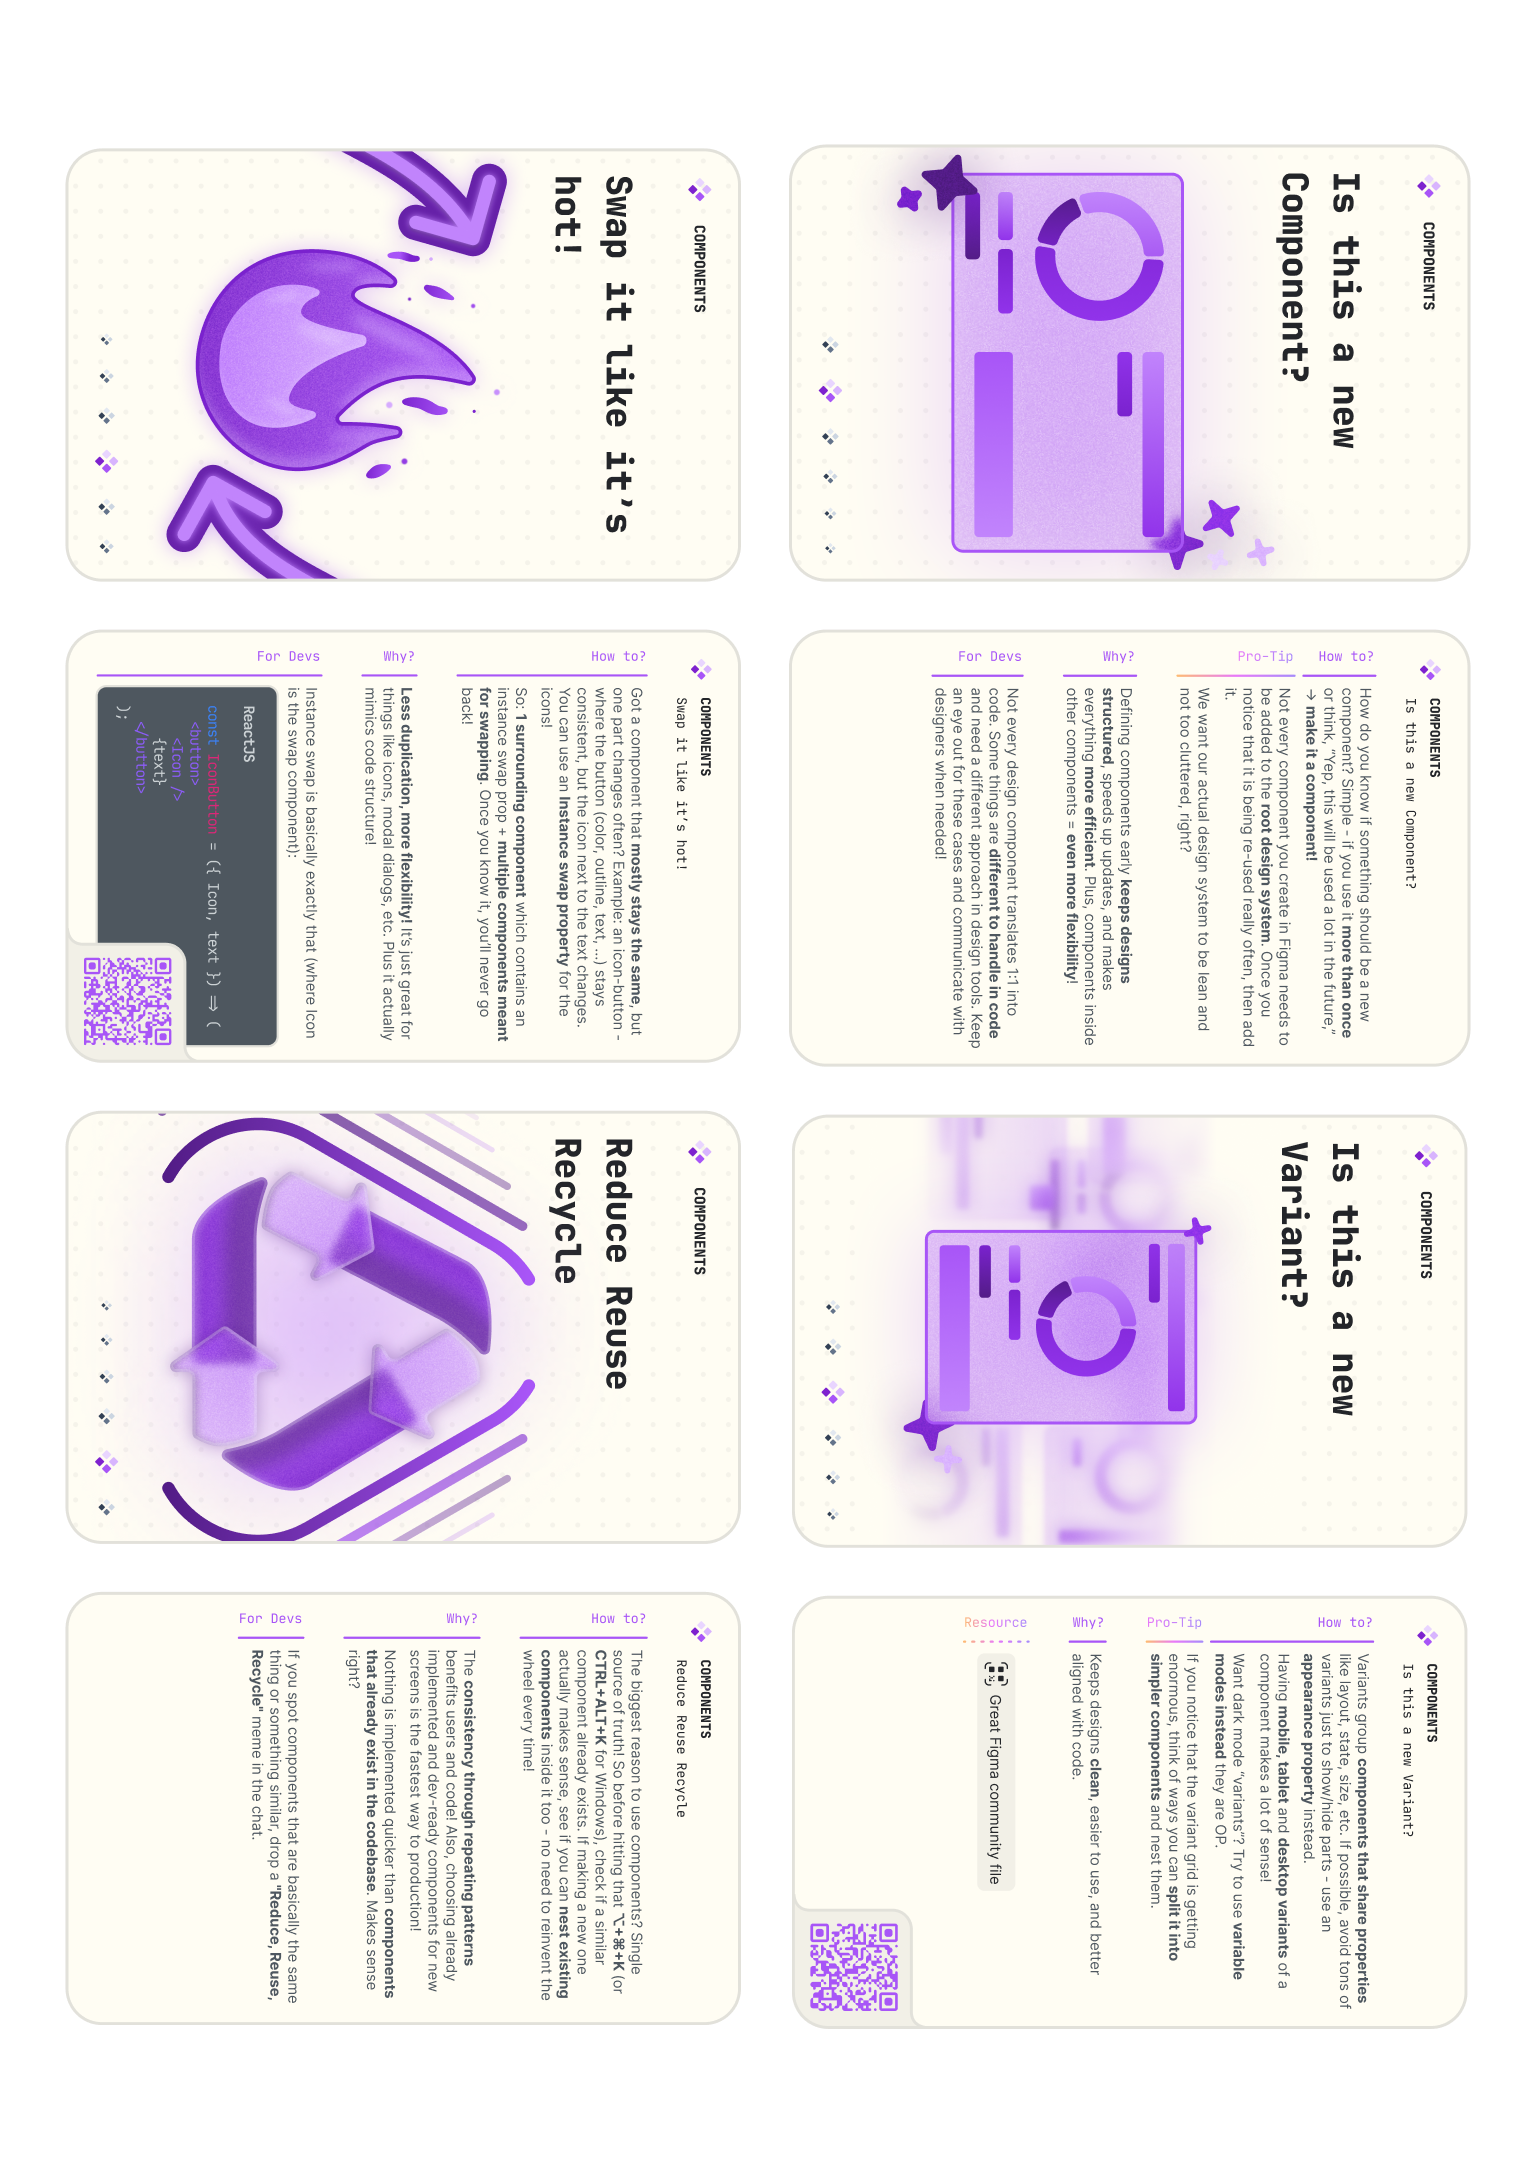
\includegraphics[width=400pt]{Chapter 5/Cards 3.png}
    \caption{The DesignAPI: Cards 3 (Source: own illustration)}
\end{figure}

\begin{figure}[H]
    \centering
    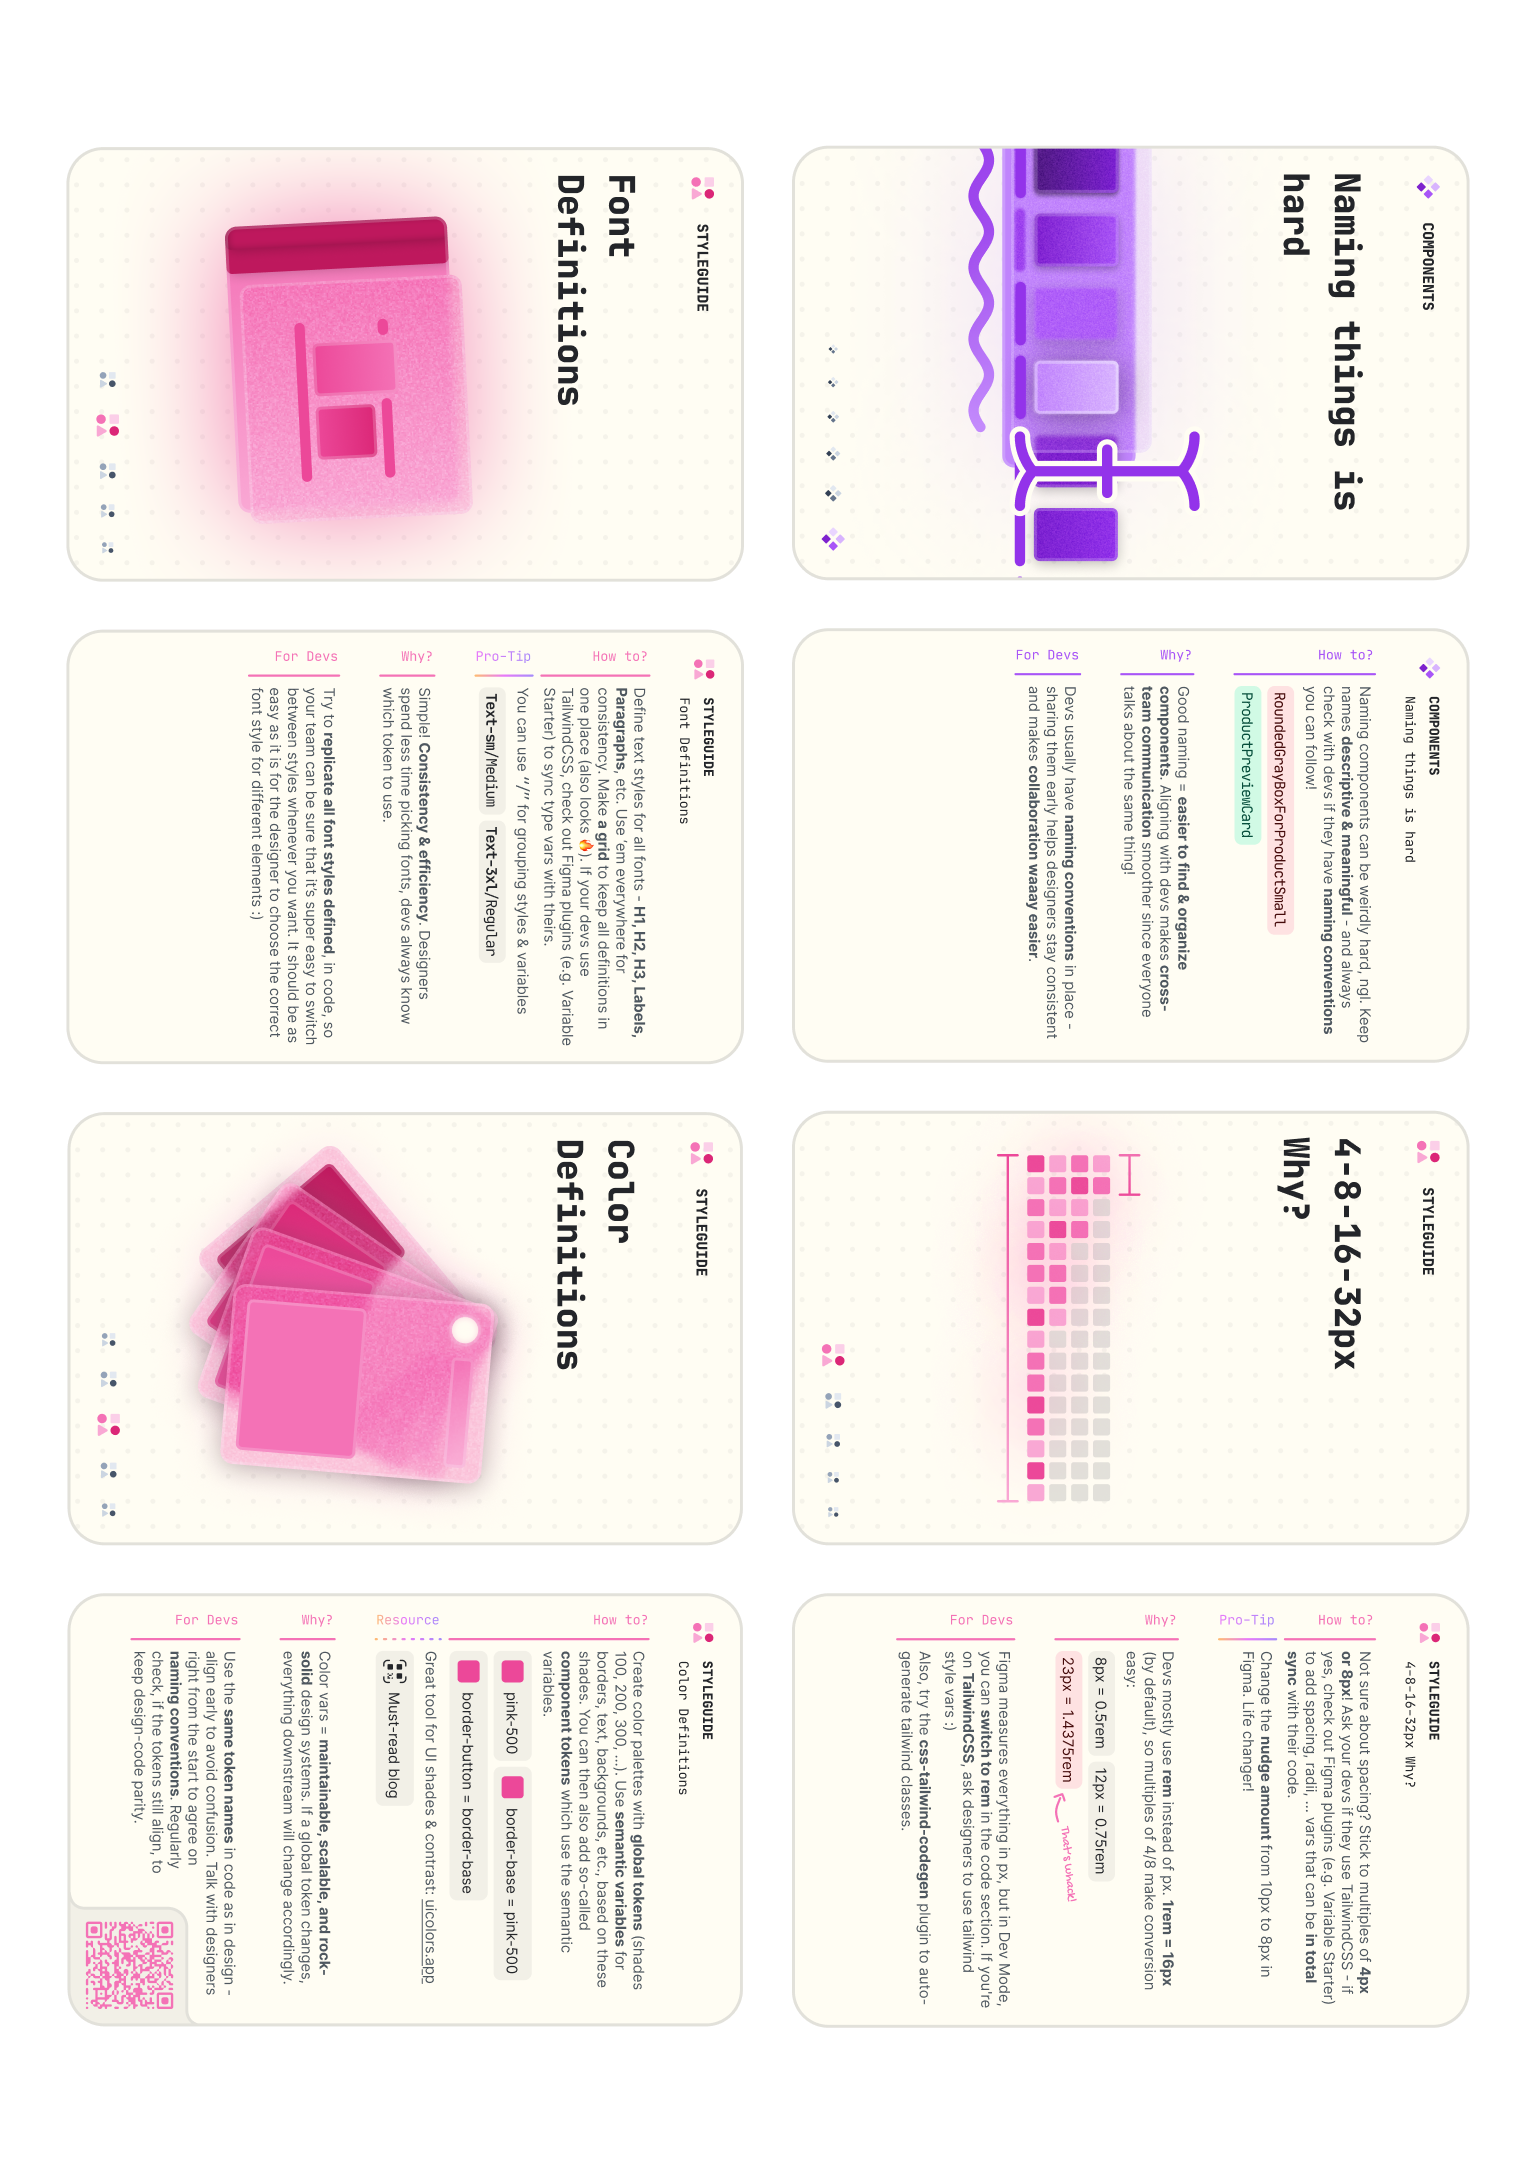
\includegraphics[width=400pt]{Chapter 5/Cards 4.png}
    \caption{The DesignAPI: Cards 4 (Source: own illustration)}
\end{figure}

\begin{figure}[H]
    \centering
    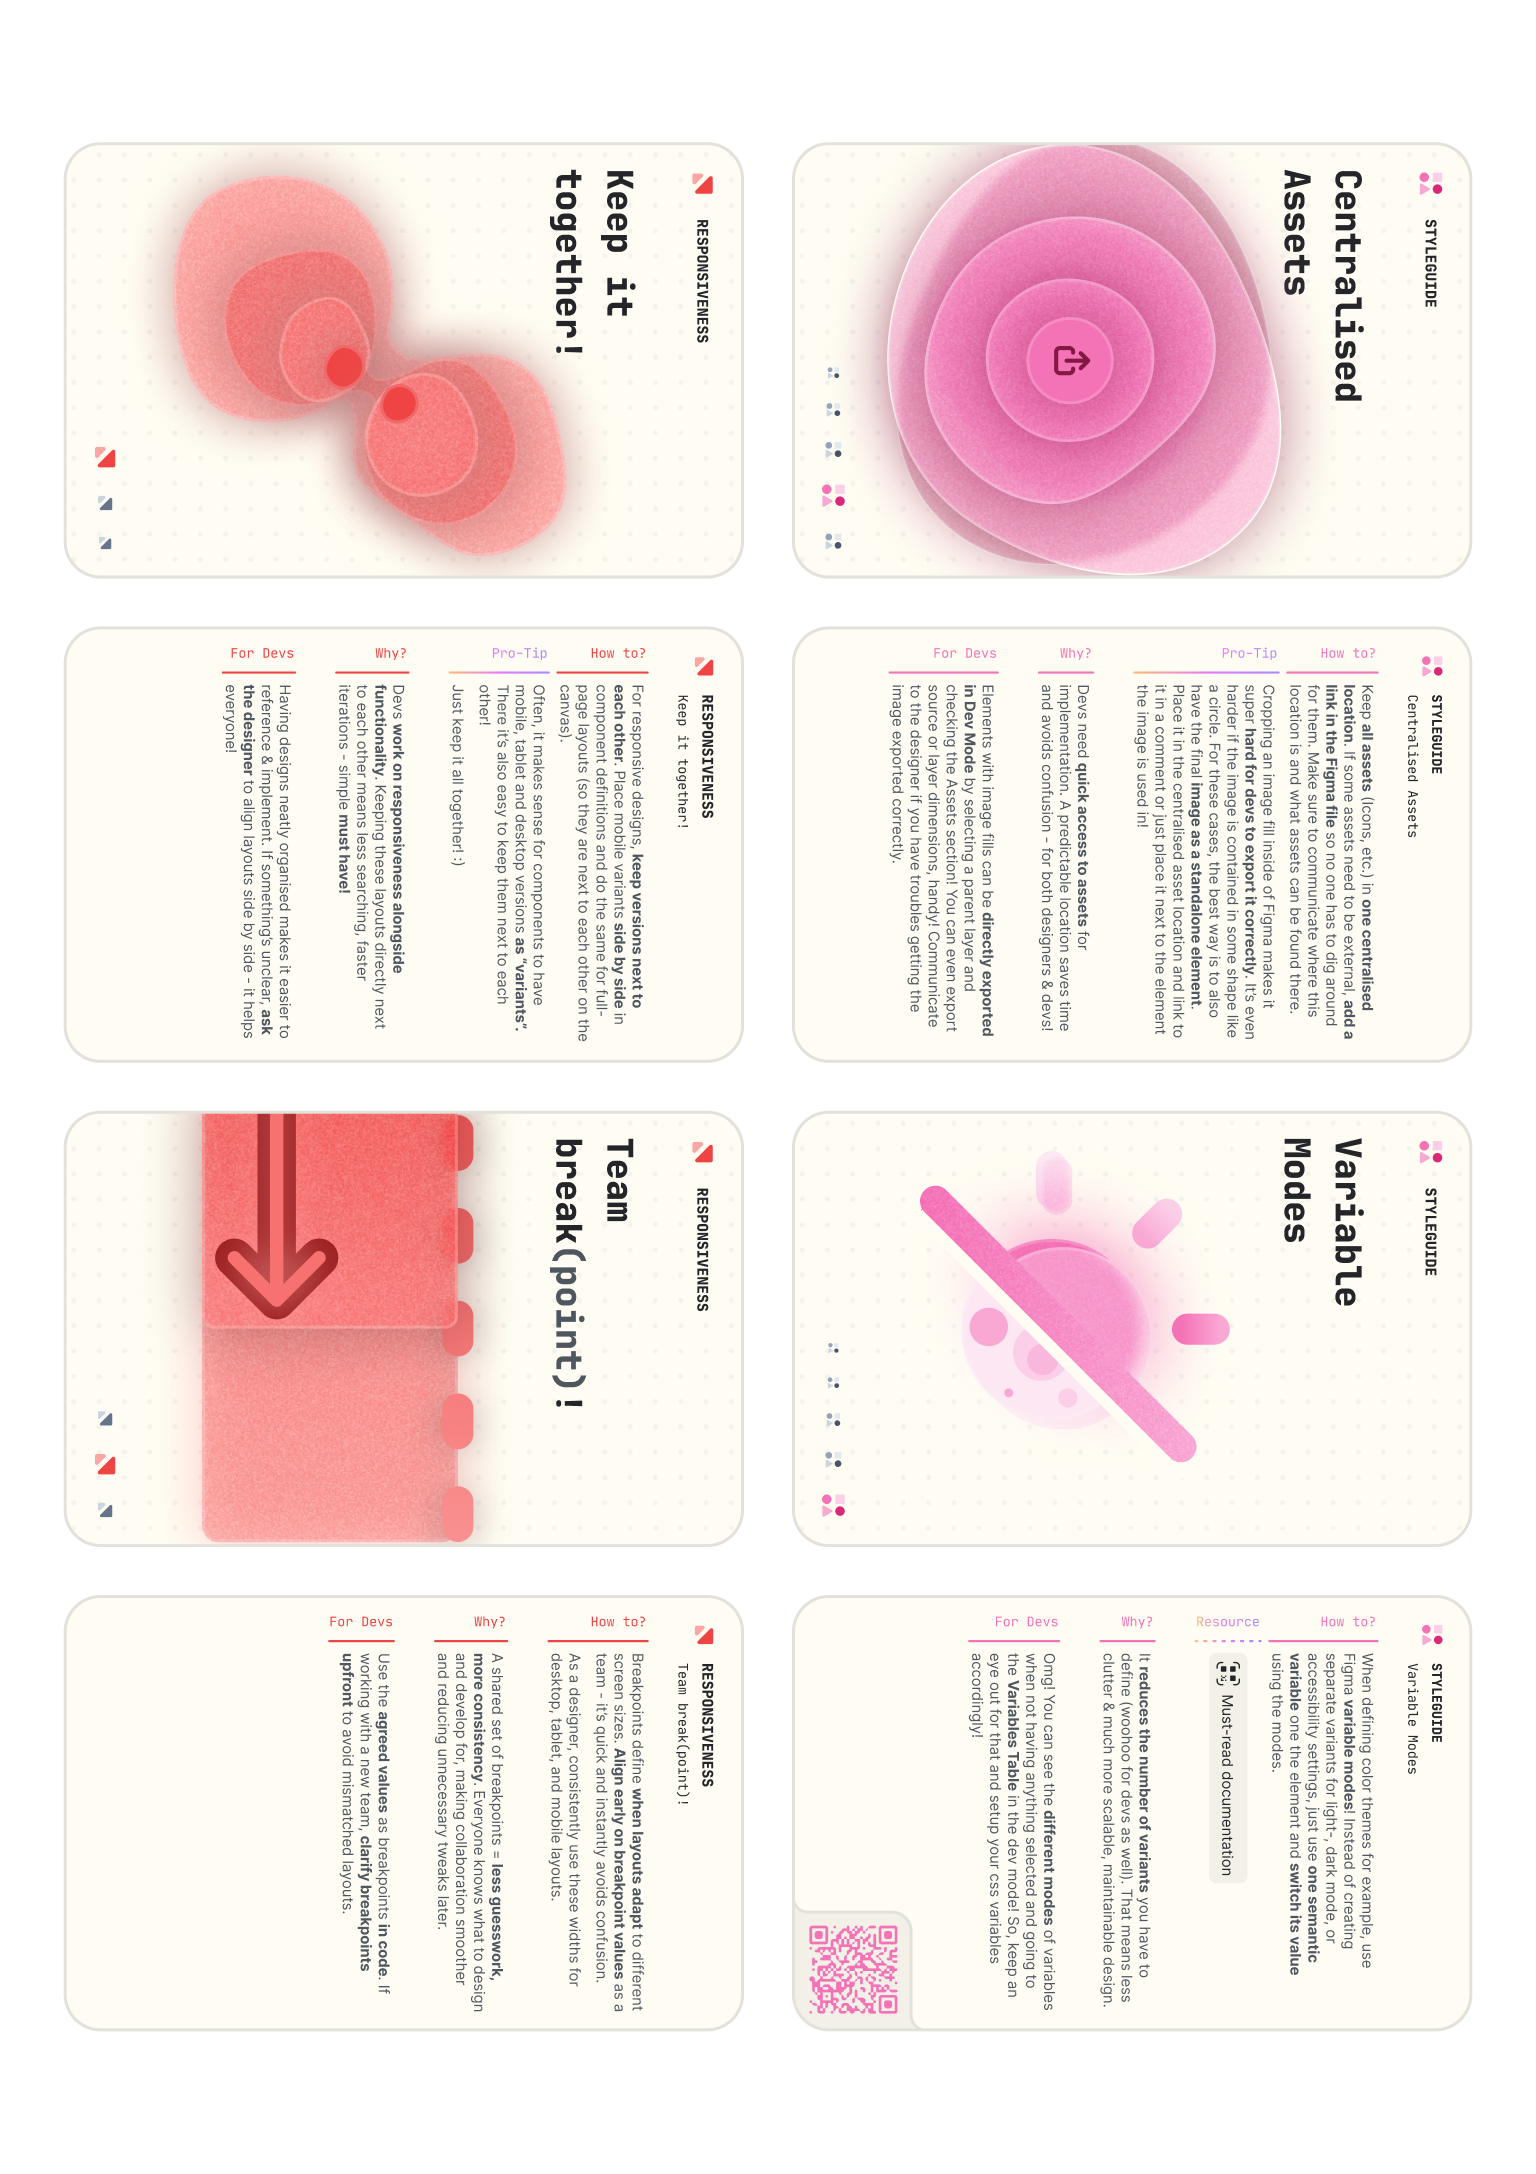
\includegraphics[width=400pt]{Chapter 5/Cards 5.png}
    \caption{The DesignAPI: Cards 5 (Source: own illustration)}
\end{figure}

\begin{figure}[H]
    \centering
    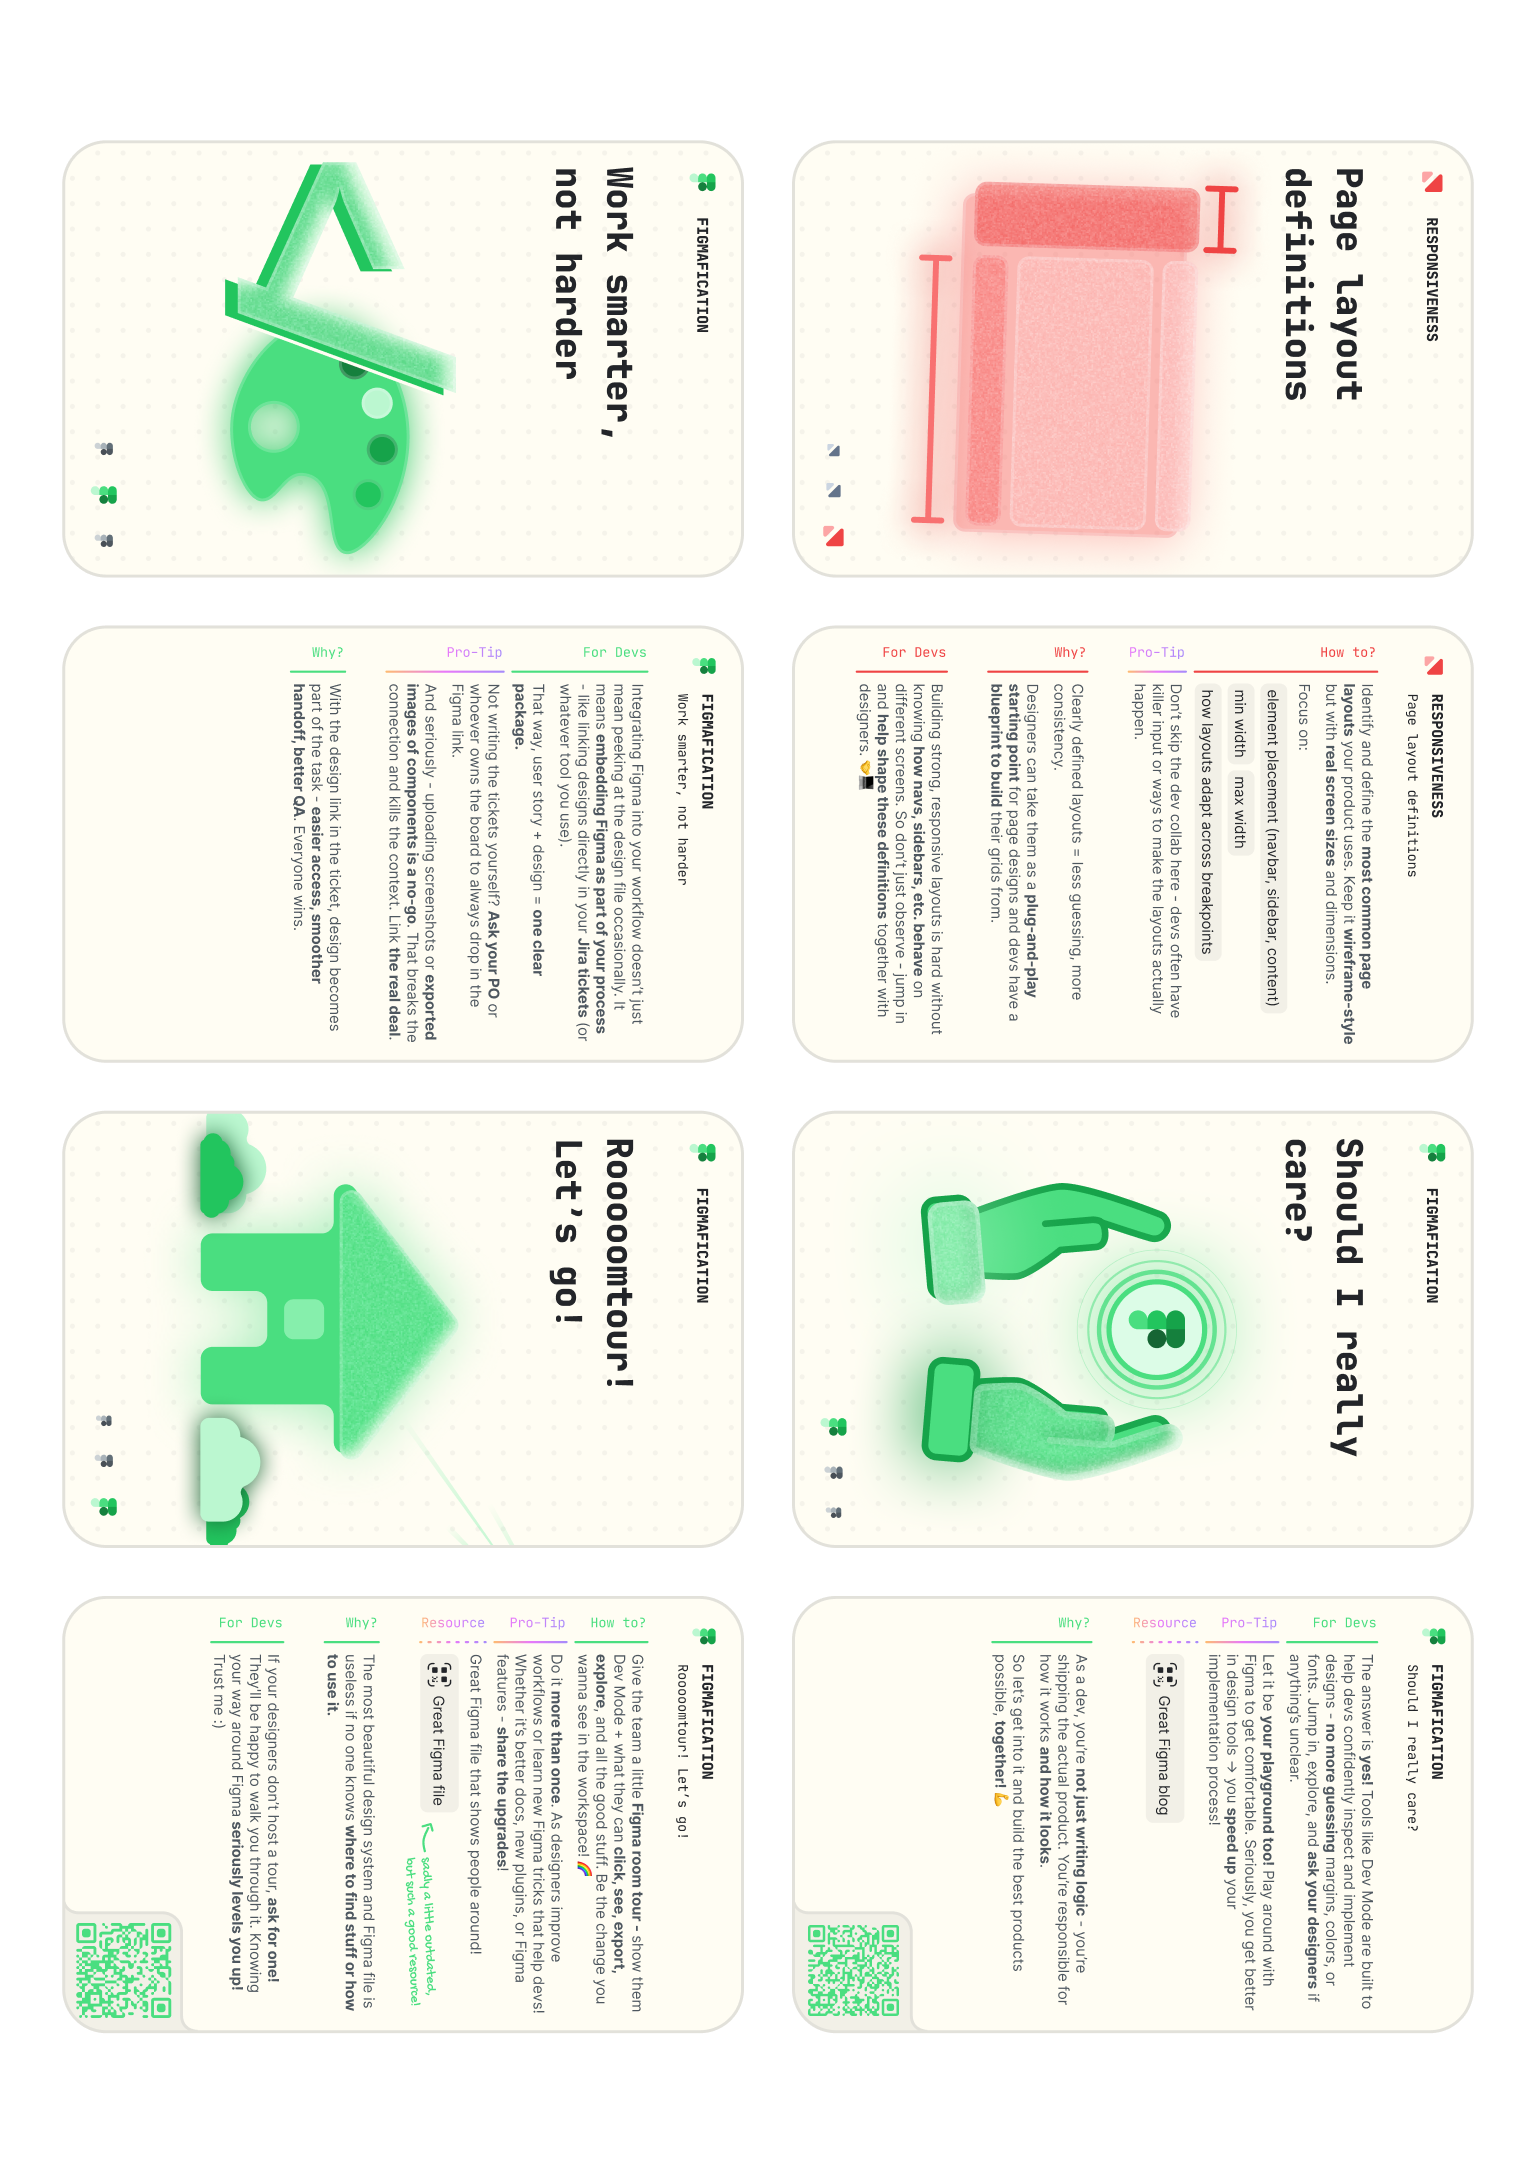
\includegraphics[width=400pt]{Chapter 5/Cards 6.png}
    \caption{The DesignAPI: Cards 6 (Source: own illustration)}
\end{figure}

\begin{figure}[H]
    \centering
    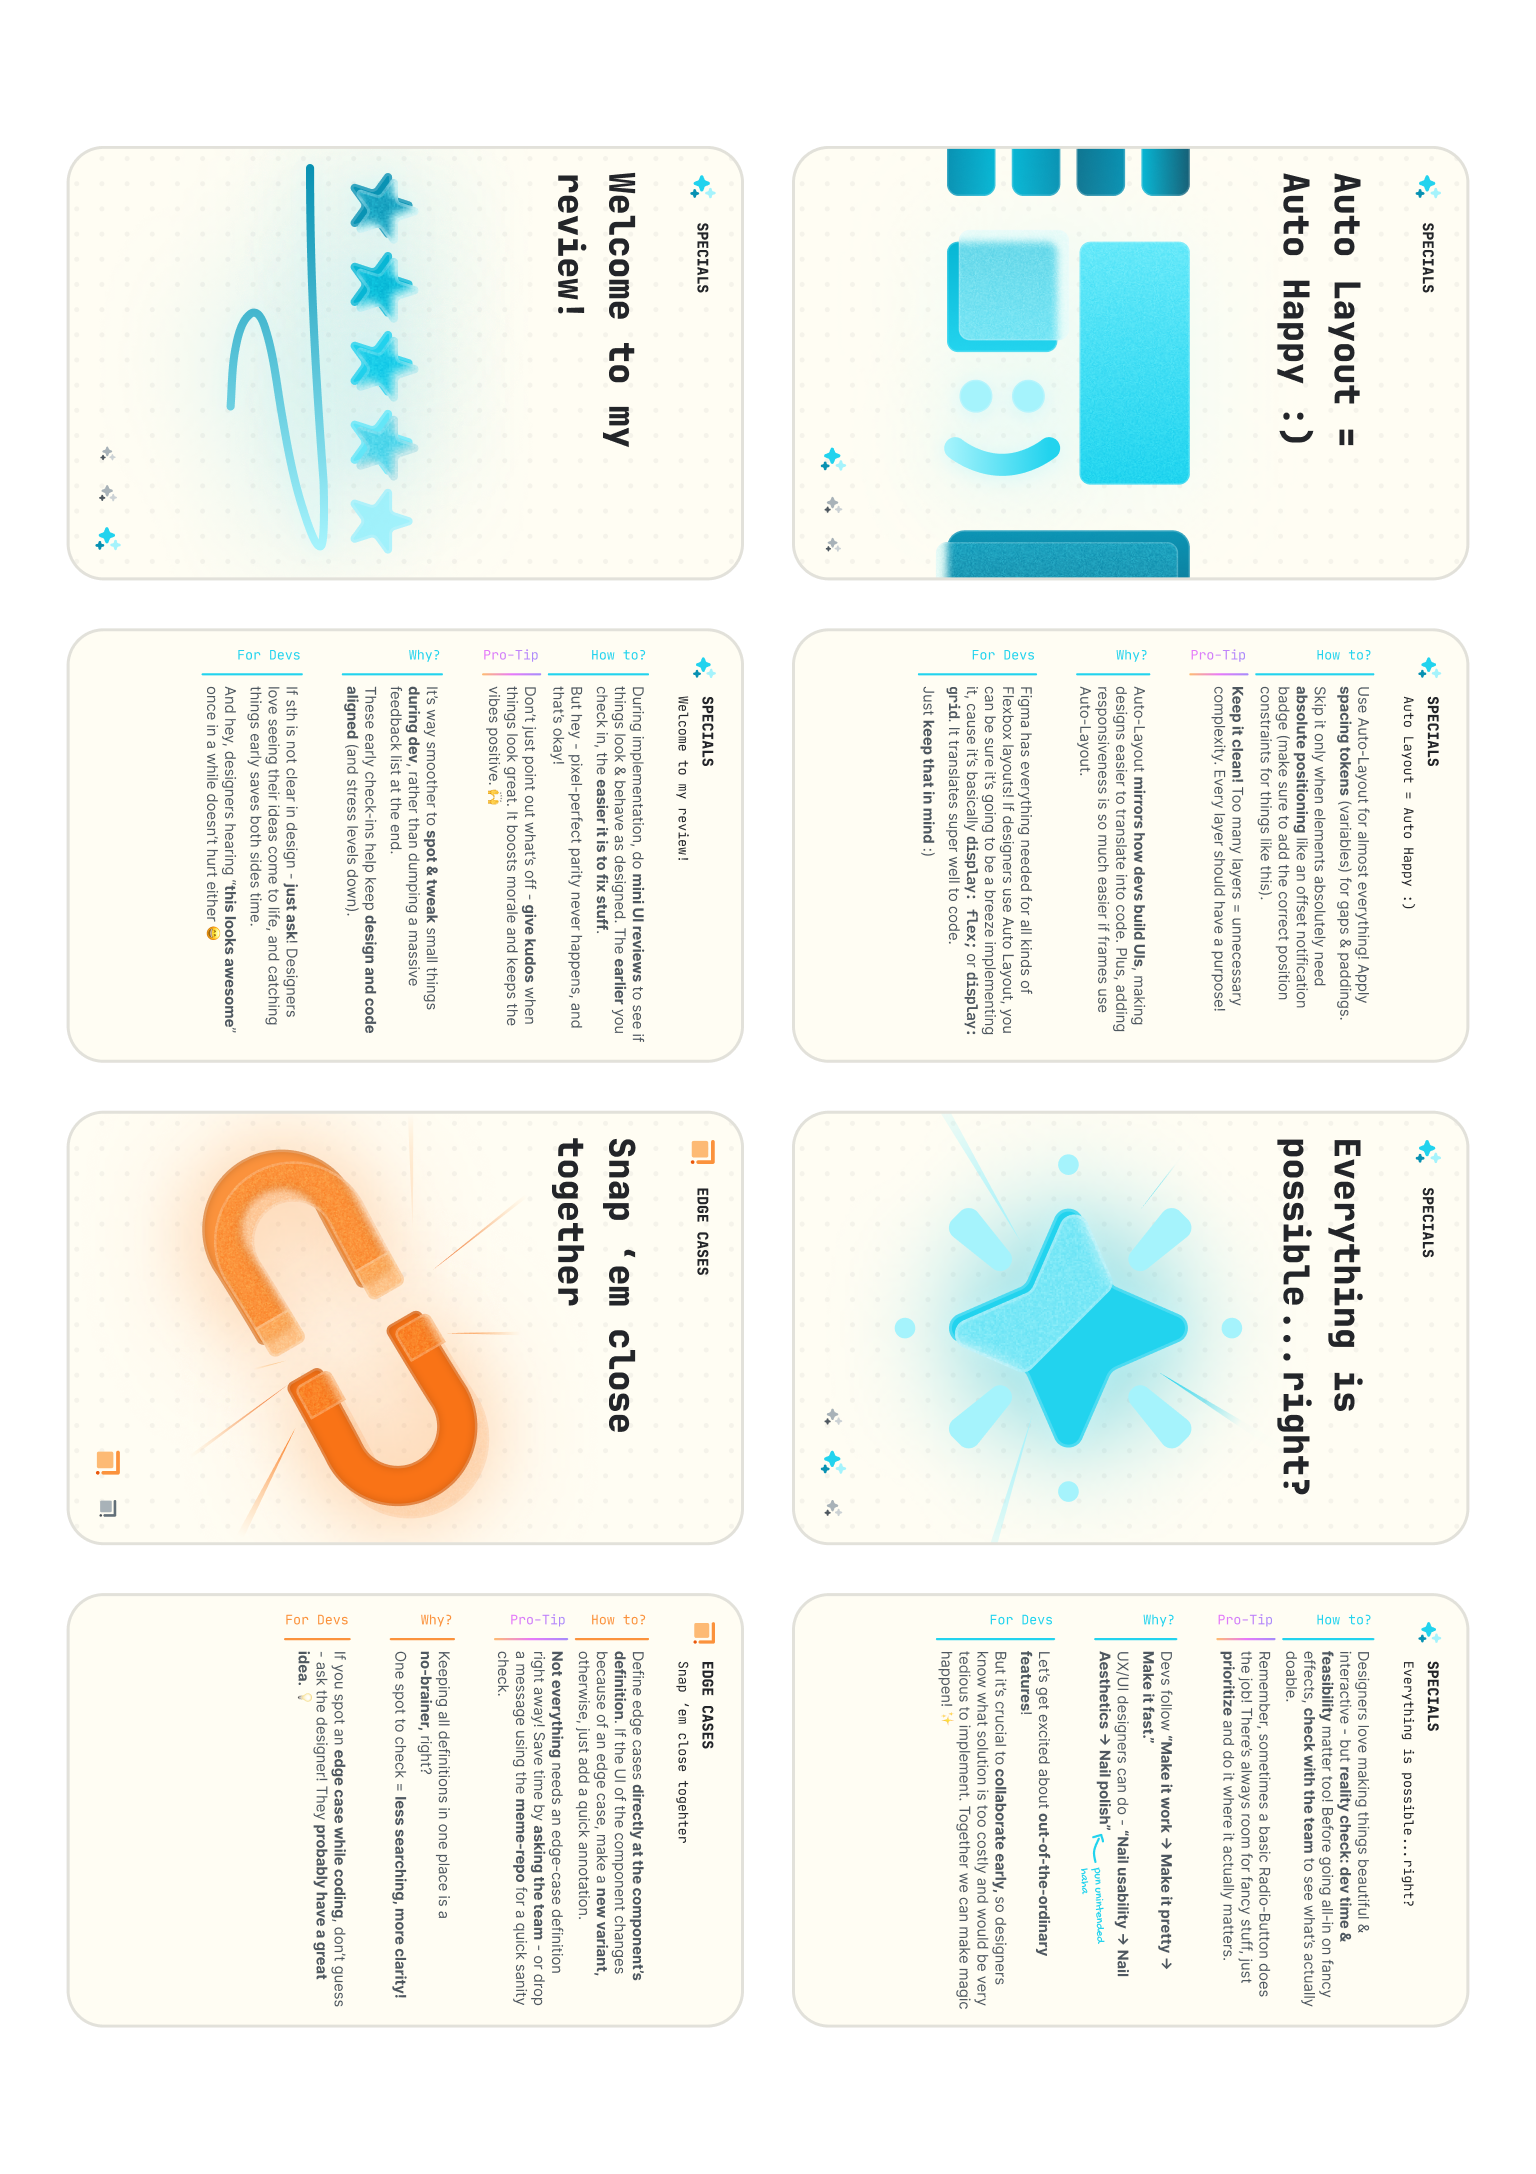
\includegraphics[width=400pt]{Chapter 5/Cards 7.png}
    \caption{The DesignAPI: Cards 7 (Source: own illustration)}
\end{figure}

\begin{figure}[H]
    \centering
    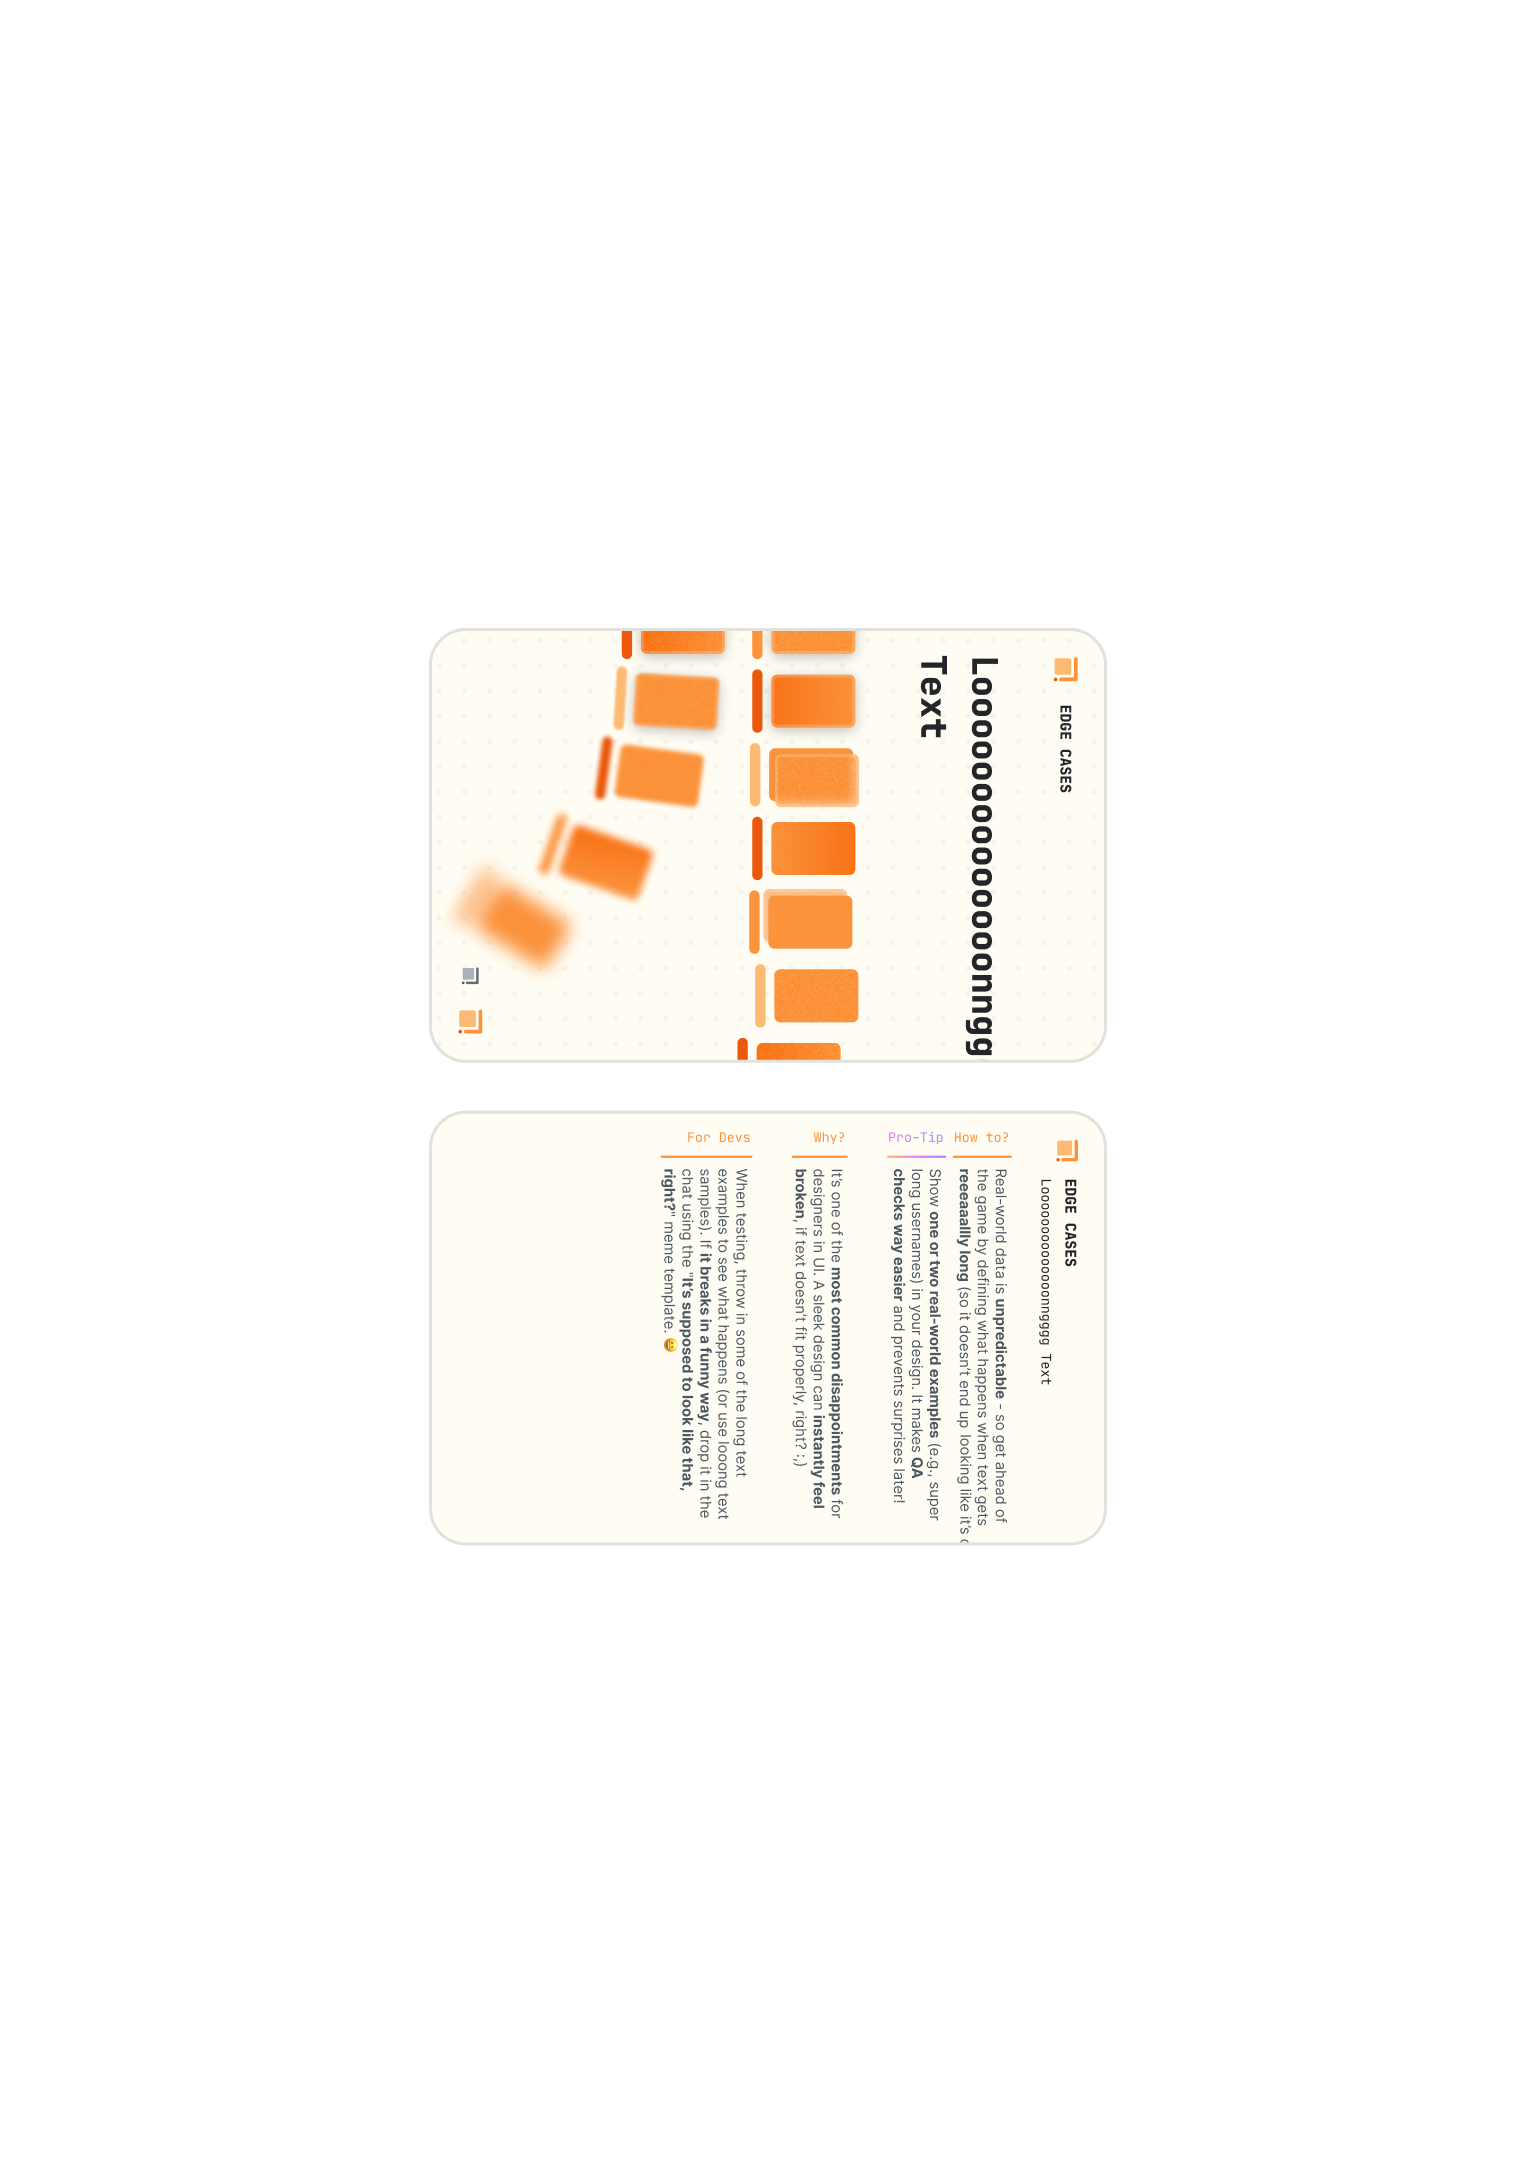
\includegraphics[width=400pt]{Chapter 5/Cards 8.png}
    \caption{The DesignAPI: Cards 8 (Source: own illustration)}
\end{figure}

\newpage
\subsection{The Message Templates}


\input{chapters/6/3_Availability.tex}


\newpage
\section{Conclusion and Afterthoughts}
The goal of this bachelor thesis was to research the most common problems in the Design-to-Code
process and to find a possible solution to conquer the majority of them. An informative card deck
with additional message templates was created, to educate and connect both disciplines.

\newpage
\subsection{Summary of the Results}
The first chapter of this thesis was all about the basics of web design. Fundamentals like user
interface design, user experience and Usability were researched and explained. Furthermore, the
world of Component Based UI design with a focus of Atomic Design was introduced and recommended best
practices were shown.

The second chapter dealt with the topic of how web projects are usually developed and answers the
question of why traditional project management is not a suitable strategy for the majority of
web projects. It shows why Agile methods in combination with Lean UX can help mitigate prevailing
issues and how close collaboration between design and development can enhance the final product. 

In the third chapter people and their experiences were in focus. A survey, with the goal of
uncovering major challenges of UI designers as well as engineers, was conducted and analyzed.
Discrepancies in the structure of UI components, lack of documentation, definition of edge cases and
misalignment in responsive design were found to be the most severe issues.

With this strong foundation, the purpose of the fourth chapter was finding a solution to these
problems. By defining a vision that would guide the practical part of this paper, the project was
systematically built by identifying the needs and creating an idea, system and design language.
Guided by experiences from the survey content for seven distinct categories was curated and written.
To be sure, that the product can truly fulfil its vision, two additional interviews were performed
with the goal of uncovering even more issues as well as obtaining feedback to the status of the
practical project. 

With another iteration, the practical work was finished and presented in chapter five titled The
DesignAPI: A Shared Interface Between Design and Code. 

\newpage
\subsection{Research Question}

\newpage
\subsection{Future Outlook}
With the DesignAPI as the output of this bachelor thesis, the next step for fulfilling its vision is
clear: Introducing it to as many design-development teams as possible. 

I hope it encourages teams to explore new ways of working together, motivated to learn from each
other and sharing a desire to improve their culture and cross-disciplinary connection.

I believe the idea of a shared interface can meaningfully boost collaboration and further
iteration will only strengthen its impact.

I know that the vision of perfect Design-to-Code processes is not just aspirational, but becoming
reality.


% =============== CHAPTERS ===============



% =============== REFERENCES ===============
\newpage
\printbibliography

\newpage
\listoffigures
% =============== REFERENCES ===============
\end{document}
